\chapter{اختصاص منابع پردازشی در شبکه اینترنت اشیاء به صورت یک به یک}\label{chap:one_to_one_allocation}
  \thispagestyle{empty}
  \section{مقدمه}
    در این فصل ابتدا مدل ریاضی مربوط به تخصیص منابع پردازشی به صورت یک به یک در شبکه‌ی اینترنت اشیاء را شرح می‌دهیم. 
    در این نوع تخصیص منابع تعدادی سرویس و منبع پردازشی داریم که سرویس‌ها باید برای پردازش داده‌های جمع‌آوری شده توسط حسگر‌های خود از منابع پردازشی موجود در شبکه استفاده کنند.
    یکی به یک بودن در این نوع تخصیص منابع به این معنی است که هر سرویس حداکثر می‌تواند از یک منبع پردازشی استفاده کند و هر منبع پردازشی می‌تواند تنها پردازش لازم برای یک سرویس را انجام دهد.
    پس از معرفی و فرمول بندی مسئله، چالش‌ها و دلایل پیچیدگی حل این مسئله را بررسی مي‌کنیم.
    سپس به معرفی راه‌حل مبتنی بر مزایده برای این مسئله می‌پردازیم.
  \section{مدل سیستم}
    \begin{figure}[h]
      \centerline{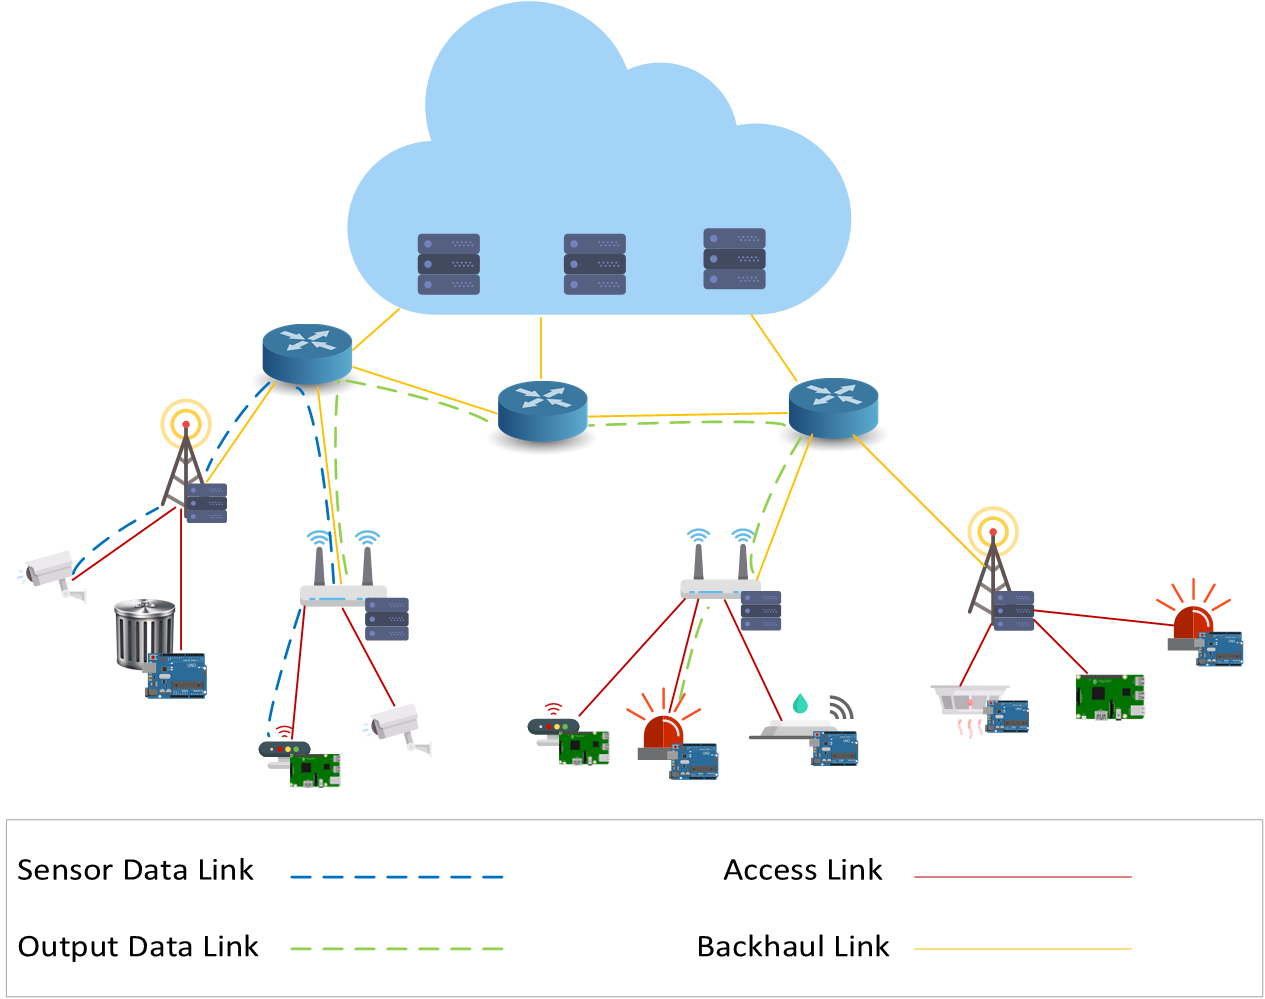
\includegraphics[width=12cm]{graphics/one_to_one/system_model}}
      \caption{دید کلی از مدل سیستم}
      \label{fig:ono_to_one_system_model}
    \end{figure}

    در یک منطقه جغرافیایی تعداد $N$ عدد سرویس و $M$ عدد فراهم کننده زیرساخت\LTRfootnote{Infrastructure Provider} پردازشی در نظر گرفته می‌شود.
    مجموعه سرویس‌ها را با $S$ و مجموع منابع پردازشی را با $C$ نمایش می‌دهیم.
    فراهم‌کننده‌های زیرساخت علاقه دارند که توان پردازشی اضافی خود را با دیگران به اشتراک بگذارند.
    در این فصل از $\phi_i$ برای بیان توان پردازشی فراهم‌کننده زیرساخت $i$ و از $\nu_i$ برای بیان درصدی از توان پردازشی که فراهم‌کننده زیرساخت پردازشی $i$ مایل به اشتراک‌گذاری آن است، استفاده می‌کنیم.
    در نتیجه، فراهم‌کننده زیرساخت پردازشی $i$ام، مایل به اشتراک‌گذاری توان پردازشی برابر با $\varphi_i = \phi_i \nu_i$ خواهد بود.
    در اینجا، گره‌های لبه\LTRfootnote{Edge Nodes}، گره‌هایی هستند که زیرساخت پردازشی را در لبه شبکه فراهم می‌کنند.
    در مقابل، فراهم‌کننده‌های زیرساخت ابری، منابع پردازشی را در فاصله‌ای دورتر از سرویس‌ها فراهم می‌کنند.
    بنابراین،‌ گره‌های لبه، توان پردازشی کم‌تر با تاخیر کم‌تر را در مقایسه با فراهم‌کننده‌های زیرساخت ابری مهیا می‌کنند.
    بده‌بستان، بین میزان توان پردازشی و تاخیر در پردازش، باعث پیچیده‌شدن انتخاب گره‌های پردازشی برای سرویس‌ها می‌شود.
    
    \cref{tbl:one_to_one:notation} به صورت خلاصه پارامتر‌ها و متغیر‌های استفاده شده در این فصل را معرفی می‌کند.
    \begin{table}[h]
      \caption{نماد‌های استفاده شده در این فصل}
      \begin{tabularx}{\textwidth}{|c|C|} \hline
        نشانه                & توضیح                                                                                     \\ \hline
        $N$                  & تعداد سرویس‌های شبکه                                                                       \\ \hline
        $M$                  & تعداد منابع پردازشی شبکه                                                                  \\ \hline
        $S$                  & مجموعه‌ی سریس‌های شبکه                                                                      \\ \hline
        $C$                  & مجموعه‌ی منابع پردازشی شبکه                                                                \\ \hline
        $d_{i,s}^\text{CPU}$ & تاخیر پردازشی سرویس $s$ در صورتی که از منبع پردازشی $i$ استفاده کند                       \\ \hline
        $d_{i,s}^\text{net}$ & تاخیر انتقال داده‌ها سرویس $s$  در صورتی که از منبع پردازشی $i$ استفاده کند                \\ \hline
        $\mu_{i,s}$         & نرخ سرویس منبع پردازشی $i$ برای سرویس $s$                                                  \\ \hline
        $r_s$               & نرخ انتخابی ارسال نمونه‌های سرویس $s$                                                       \\ \hline
        $R_s$               & نرخ مطلوب ارسال نمونه‌ها برای سرویس $s$                                                     \\ \hline
        $\omega_s$          & ضریب وزن دهی برای مشخص کردن نسبت اهمیت تاخیر نسبت به اختلاف نرخ انتخابی و نرخ مطلوب برای سرویس‌ها \\ \hline
        $\delta_{i,s}$      & متغیر دودویی که مشخص می‌کند سرویس $s$ منبع پردازشی $i$ را استفاده می‌کند یا خیر              \\ \hline
        $f_r$               & تابع مشخص کننده تاثیر اختلاف نرخ انتخابی با نرخ مطلوب در ارزش سرویس                         \\ \hline
        $f_d$               & تابع مشخص کننده تاثیر تاخیر در ارزش سرویس                                                  \\ \hline
        $U_{i,s}$           & ارزش سرویس $s$ در صورتی که از منبع پردازشی $i$ استفاده کند                                 \\ \hline
        $U_s$               & ارزش سرویس $s$                                                                             \\ \hline
        $U$                 & مجموع ارزش سرویس‌ها                                                                         \\ \hline
        $\eta$              & پارامتر محدود کننده‌ی بهره برداری از منابع پردازشی                                          \\ \hline
        $\epsilon$          & حداقل مقدار افزایش قیمت منابع پردازشی توسط سرویس‌ها در هر پیشنهاد                           \\ \hline
        $p_i$               & قیمت استفاده از منبع پردازشی $i$                                                           \\ \hline
        $\iota_s$           & منبع پردازشی با بیش‌ترین سود برای سرویس $s$                                                 \\ \hline
        $v_s$               & سود بهترین منبع پردازشی برای سرویس $s$                                                     \\ \hline
        $w_s$               & سود دومین بهترین منبع پردازشی برای سرویس $s$                                               \\ \hline
        $\gamma_s$          & میزان افزایش قیمت برای بهترین منبع پردازشی سرویس $s$                                       \\ \hline
      \end{tabularx}
      \label{tbl:one_to_one:notation}
    \end{table}

    در ابتدا تاخیر سرویس‌ها را بررسی می‌کنیم.
    تاخیر سرویس $s$ زمانی که از منبع پردازشی $i$ استفاده می‌کند، از دوبخش تشکیل می‌شود.
    یکی مربوط به تاخیر شبکه‌ است که آن را با $d^\text{net}$ نمایش می‌دهیم.
    دیگری مربوط به تاخیر پردازش است که آن را با $d^\text{CPU}$ نمایش می‌دهیم.
    تاخیر شبکه ($d^\text{net}$) زمانی است که لازم است تا حسگر‌‌های یک سرویس داده‌ها رو برای منبع پردازشی اختصاص یافته ارسال کنند به علاوه زمانی که لازم است تا گره پردازشی نتیجه را برای مقصد ارسال کند.
    تاخیر پردازشی ($d^\text{CPU}$) زمانی است که طول می‌کشد تا داده‌ها در منبع پردازشی، پردازش شوند.
    
    در این‌جا فرض می‌کنیم که تاخیری شبکه ثابت است و تنها تابع فاصله جغرافیایی و ادوات شبکه بین فرستنده و گیرنده است.
    همانند \cite{optimial_price_cloud_valerio} از تئوری صف برای مدل کردن تاخیر پردازشی استفاده می‌کنیم.
    در این روش، پردازنده مانند یک سرویس دهنده عمل می‌کند و درخواست‌ها در یک صف قرار می‌گیرند تا نوبت پردازش آن‌ها فرار برسد.
    چون در این فصل هر گره پردازشی تنها به یک سرویس اختصاص پیدا می‌کند، از مدل $M/D/1$ استفاده می‌کنیم.
    در این مدل، فرایند ورود به صف بدون حافظه بوده و نرخ سرویس‌ مقدار ثابتی دارد.
    برای یک صف $M/D/1$ با نرخ ورود $\lambda$ و نرخ سرویس  $\mu$ میانگین تاخیر $\omega$ از رابطه زیر بدست می‌آید\cite{basic_queueing_sztrik}
    \begin{equation}\label{eqn:md1_queue_responsetime}
      \omega = \frac{1}{\mu} + \frac{\lambda}{2\mu(\mu-\lambda)}.
    \end{equation}
    
    نرخ ارسال نمونه‌های حسگر‌های سرویس $s$ را $r_s$ می‌نامیم.
    در این صورت نرخ ورود در مدل $M/D/1$ برای منبع پردازشی $i$ برابر $r_s$ خواهد بود.
    همان‌گونه که قبلا توضیح داده شد، $\varphi_i$ بیان‌گر ضرفیت پردازشی است که منبع پردازشی $i$ مایل به اشتراک گذاری آن است.
    این عدد در واقع تعداد دستور العمل‌های پردازنده مرکزی\LTRfootnote{CPU Instructions} که این منبع پردازشی در یک ثانیه می‌تواند اجرا کند را بیان می‌دارد.
    اگر فرض کنیم $F_s$ تعداد دستور العمل‌های لازم برای پایان یافتن پردازش‌های یک نمونه از داده‌های حسگر های سرویس‌ $s$ را نشان دهد، نرخ سرویس منبع پردازشی $i$ برای سرویس $s$ از رابطه زیر بدست می‌آید
    \begin{equation}
      \mu_{i,s} = \frac{\varphi_i}{F_s}.
    \end{equation}
    با جایگذاری این مقدار در \cref{eqn:md1_queue_responsetime} تاخیر پردازشی سرویس $s$ وقتی از منبع پردازشی $i$ استفاده می‌کند به صورت زیر دست می‌آید:
    \begin{equation}
      d_{i,s}^{\text{CPU}} = \frac{2\mu_i-r_s}{2\mu_i(\mu_i-r_s)}.
    \end{equation}

    در این جا فرض می کنیم که ارزش منبع پردازشی $i$ برای سرویس $s$ از دو بخش تشکیل شده است.
    بخش اول، تابع نرخ ارسال نمونه‌ها توسط حسگر‌های سرویس $s$ به منبع پردازشی $i$ است.
    این تابع را $f_r$ نام‌گذاری می‌کنیم و فرض می‌کنیم که $f_r$ تابعی از نرخ ارسال نمونه‌ها توسط حسگر‌های سرویس $s$ و نرخ مطلوب آن سرویس می‌باشد.
    در واقع $f_r$ بیان کننده‌ی تا ثیر $r_s$ در ارزش بدست آمده از پردازش اطلاعات برای سرویس‌ها است.
    بخش دوم هم تابعی از تاخیر ایجاد شده (مجموع تاخیر شبکه و تاخیر پردازش) است که آن را با $f_d$ نمایش می‌دهیم.
    اگر فرض کنیم $R_s$ نرخ ارسال مطلوب سرویس $s$ و $r_s$ نرخی باشد که آن سرویس تصمیم می‌گیرد با آن نرخ نمونه‌ها را برای پردازش ارسال کند، ارزشی که سرویس $s$ با استفاده از منبع پردازشی $i$ بدست می‌آورد را به صورت زیر می‌توان نوشت
    \begin{equation}
      U_{i,s}(r_s) = \alpha_s \left (\omega_s f_r(r_s, R_s) + (1-\omega_s) f_d(d_{i,s}^{\text{net}} + d_{i,s}^{\text{CPU}}) \right ) .
    \end{equation}
    نکته قابل توجهه در این رابطه این است که $\omega_s \in [0,1]$ یک ضریب وزن دهنده است که تعیین کننده نسبت تاثیر $f_r$ به $f_d$ است.
    اگر $\omega = 1$ باشد ضریب $f_d$ صفر خواهد بود، در نتیجه تاخیر اثری در ارزش بدست‌آمده برای سرویس نقشی نخواهد داشت.
    اما $\omega = 0$ بیان‌گر این است که نرخ اختصاص یافته برای سرویس اهمیتی ندارد و فقط تاخیر برای سرویس مهم است.
    واضح است که اگر $\omega = 0$ باشد، نرخی که ارزشی بدست آمده برای سرویس را بیشینه می‌کند $r_s = 0$ است.
    در نتیجه $\omega = 0$ نتیجه قابل قبولی نخواهد داشت.
    $\alpha_s$ برای اثر دادن ارزش ذاتی سرویس‌ها است.
    پس $\alpha_s$ برای سرویس با ارزش بالاتر، باید مقدار بیشتری داشته باشد.
    در ادامه برای نشان دادن اختصاص منبع پردازشی $i$ به سرویس $s$ از $\delta_{i,s}$ که به صورت زیر تعریف می‌شود استفاده می‌کنیم
    \begin{equation*}
      \delta_{i,s} = 
      \begin{cases}
        1, & \text{اگر منبع پردازشی $i$ به سرویس $s$ اختصاص پیدا کرده باشد} \\
        0, & \text{در غیر این صورت}
      \end{cases}.
    \end{equation*}
    با این تعریف ارزش بدست آمده برای سرویس $s$ از تخصیص منابع را می‌توان به صورت زیر بیان کرد
    \begin{equation}
      U_{s} =  \alpha_s \left (\omega_s  f_r(r_s, R_s) + (1-\omega_s) \sum_{i=1}^M \delta_{i,s} f_d(d_{i,s}^{\text{net}} + d_{i,s}^{\text{CPU}}) \right).
    \end{equation}
    در این رابطه به دلیل ضرب $\delta_{i,s}$ در $f_d$ فقط $f_d$ مربوط به منبع پردازشی اختصاص یافته به سرویس $s$ در $U_s$ تاثیر گذار خواهد بود.

    هدف ما این است که تخصیص منابعی را پیدا کنیم که مجموع ارزش بدست آمده برای سرویس‌ها را بیشینه کند.
    ارزشی که همه سرویس‌ها از تخصیص منابع بدست می‌آورند را $U$ نام‌گذاری می‌کنیم که به صورت زیر تعریف می‌شود
    \begin{equation}
      U = \sum_{s=1}^N \alpha_s \left (\omega_s f_r(r_s, R_s) + (1-\omega_s) \sum_{i=1}^M \delta_{i,s} f_d(d_{i,s}^{\text{net}} + d_{i,s}^{\text{CPU}}) \right).
    \end{equation}
    در واقع $U$ تابع هدف مسئله است و می‌توانیم مسئله تخصیص منابع را به صورت مسئله بهینه سازی زیر بنویسیم
    \begin{subequations}
      \begin{align}
        \underset{r_s, \delta_{i,s}}{\text{maximize}} \qquad & \sum_{s=1}^N \alpha_s \left (\omega_s f_r(r_s, R_s) + (1-\omega_s) \sum_{i=1}^M \delta_{i,s} f_d(d_{i,s}^{\text{net}} + d_{i,s}^{\text{CPU}}) \right ) \\
        \text{\lr{subject  to}} \qquad & \nonumber \\
        & 0 \le r_s, \forall s \in S\label{eqn:rate_positiveness} \\
        & r_s \le \eta \sum_{i=1}^M \mu_{i,s}, \forall s \in S\label{eqn:rate_saturation}\\
        & \sum_{s=1}^N \delta_{i,s} \le 1, \forall i \in C \label{eqn:one_to_one:resource_quota}\\
        & \sum_{i=1}^M \delta_{i,s} \le 1, \forall s \in S \label{eqn:one_to_one:service_quota}\\
        & \delta_{i,s} \in \{0, 1\}, \forall s \in S, i \in C
      \end{align}
    \end{subequations}
    قید \eqref{eqn:rate_positiveness} بیان می‌کند که نرخ ارسال انتخاب شده برای سرویس‌ها باید مثبت باشد.
    قید \eqref{eqn:rate_saturation} برا جلوگیری از اشباع شدن منابع پردازشی است.
    در این قید، $0 < \eta < 1$ حداکثر مقدار بهره‌برداری از منابع پردازشی اختصاص یافته به سرویس‌ها را محدود می‌کند.
    نکته حائز اهمیت این است که در صف‌های $M/D/1$ واریانس تاخیر با افزایش بهره‌بردازی از منابع افزایش می‌یابد. {\xecolor{red}منبع اضافه کنم؟}
    به همین دلیل با افزایش $\eta$ واریانس تاخیر سرویس‌ها افزایش پیدا می‌کند که خود می‌تواند باعث افزایش نا اطمینانی در سرویس‌ها شود.
    در نتیجه ممکن برای بعضی سرویس‌ها لازم باشد که $\eta$ به طور جداگانه بر حسب نیازشان محاسبه شود.
    همان‌گونه که قبلا بیان شد در این فصل فرض بر این است که تخصیص منابع یک به یک است یعنی هر سرویس می‌تواند حداکثر از یک منبع پردازشی استفاده کند و هر منبع پردازشی هم حداکثر به یک سرویسی اختصاص پیدا می‌کند.
    قید‌های \eqref{eqn:one_to_one:resource_quota} و \eqref{eqn:one_to_one:service_quota} وظیفه دارند این شرایط را برقرار سازند.
        
    تابع‌های $f_r$ و $f_d$ در تابع هدف بهینه‌سازی باید شرایط خاصی داشته باشند تا بتوان آن‌ها را مورد قبول دانست.
    $f_r$ باید تابع اختلاف $r_s$ و $R_s$ باشد و با افزایش این اختلاف، مقدار آن کاهش پیدا کند.
    $f_d$ هم باید با افزایش تاخیر‌ کاهش پیدا کند.
    در ادامه‌ی این فصل فرض می‌کنیم:
    \begin{latin}
      \begin{itemize}
        \item $f_r(r_s, R_s) = -|R_s - r_s|$
        \item $f_d(d^\text{CPU}_{i,s} + d^\text{net}_{i,s}) = - d^\text{CPU}_{i,s} - d^\text{net}_{i,s}$
      \end{itemize}
    \end{latin}
    واضح است که این توابع، شرایطی که در بالا بیان شده است را دارند.
    {\xecolor{red}دوباره مسئله بهینه سازی رو بنویسم؟}

    مسئله بهینه سازی معرفی شده در این بخش یک مسئله برنامه‌ریزی غیرخطی عدد صحیح مخلوط \LTRfootnote{Mixed Integer Nonlinear Programming} می‌باشد.
    این نوع مسائل به طور کلی به سختی حل می‌شوند \cite{bertsimas1997introduction}.
    تعداد زیاد متغیر‌های موجود در این مسئله به دلیل تعداد فراوان سرویس‌ها و منابع پردازشی در سناریو‌های مربوط به اینترنت اشیاء پیدا کردن جواب بهینه این مسئله را غیر عملی می‌کنند.
    به همین دلیل یک جواب زیر بهینه که به صورت عملی قابل محاسبه باشد مطلوب است.
    در بخش بعدی روشی مبتنی بر مزایده را معرفی می‌کنیم که پاسخ زیر بهینه این مسئله را به صورت عملی محاسبه می‌کند.

  \section{تخصیص منابع با استفاده از مزایده}
    در روش‌ تخصیص منابع مبتنی بر مزایده فرض می‌شود که یک سرویس باید مقدار پول $p_i$ را به منبع $i$ بپردازد تا بتواند از آن استفاده کند.
    در این روش برای هر سرویس سود را اختلاف بین ارزشی که آن منبع برای سرویس ایجاد می‌کند و پولی که برای بدست آوردن آن پرداخت می‌کند، تعریف می‌کنیم.
    از این رو هرکدام از سرویس‌ها تلاش می‌کنند تا منبعی را بدست بیاورند که بیشترین سود را برای آن‌ فراهم می‌کند.
    باید توجه داشت که در این جا منظور از منابع منابع، همان منابع پردازشی می‌باشد.
    \subsection{مروری بر روش مزایده}
      اگر $\iota_s$ منبعی باشد که بیشترین سود را برای سرویس $s$ فراهم کند، در این صورت رابطه زیر برای سرویس $s$ و منابع پردازشی برقرار خواهد بود:
      \begin{align}\label{eqn:maximal_net_value}
        U_{\iota_s,s} - p_i \ge \max_i \{U_{i,s} - p_i\}.
      \end{align}
      اگر \cref{eqn:maximal_net_value} برای همه سرویس‌ها برقرار باشد، به آن تعادل اقتصادی\LTRfootnote{Economic Equilibrium} می‌گویند\cite{auction_algorithms_bertsekas}.
      {\xecolor{red}در این نوع تعادل، تمام طرف‌های درگیر، از منابع اختصاص یافته راضی هستند چرا که هیچکدام نمی‌توانند سود خود را افزایش دهند.}
      در نتیجه هیچ‌کس انگیزه‌ای برای تغییر منابع اختصاص یافته ندارد.
      با این وجود، پیدا کردن این تعادل عملی نیست.
      دلیل عملی نبودن پیدا کردن این تعادل این است که حالت‌هایی وجود دارد که در {\xecolor{red}{فرایند}} پیدا کردن این تعادل حلقه به وجود می‌آید و فرایند خاتمه پیدا نمی‌کند.
      به عبارت دیگر حالت‌هایی ممکن است وجود داشته باشد که دو یا چند سرویس، ارزش یکسانی برای تعدادی از منابع قائل باشند.
      این حالت مانع افزایش قیمت منابع می‌شود.
      در نتیجه فرایند حراج هیچ وقت پایان نمی‌یابد.
      برای حل این مشکل، \cite{auction_algorithms_bertsekas} الگوریتمی ارائه کرد که تلاش می‌کند یک تعادل تقریبی\LTRfootnote{Almost Equilibrium} راپیدا کند.
      
      در یک تعادل تقریبی، تفاوت بین سود هریک از سرویس‌ها از بهینه بودن،باید حداکثر به اندازه‌ی $\epsilon$ باشد.
      در نتیجه در یک تعادل تقریبی رابطه زیر برای همه سرویس‌ها برقرار است
      \begin{equation}\label{eqn:almost_equilibrium}
        U_{\iota_s,s} - p_i \ge \max_i \{U_{i,s} - p_i\} - \epsilon.
      \end{equation}
      این رابطه برای هر سرویسی که برقرار باشد آن سرویس تقریبا راضی است.
      در واقع آن سرویس با تغییر منبعی که انتخاب کرده نمی‌تواند سود خود را بیشتر از $\epsilon$ افزایش دهد.
      این شرط با نام \lr{$\epsilon$ - complementary~slackness} شناخته می‌شود و در صورتی که $\epsilon = 0$ باشد، نتایج مانند تعادلی که توسط \cref{eqn:maximal_net_value} معرفی شد خواهد داشت.
      الگوریتم معرفی شده، یک روش مبتنی بر تکرار است که بالاخره یک تعادل تقریبی را پیدا می‌کند.

      در ابتدا هرکدام از سرویس‌ها منبع پردازشی که بیشترین سود را برایش فراهم می‌کند انتخاب می‌کند.
      همان طور که قبلا هم بیان شد، $\iota_s$ بهترین منبع پردازشی را برای سرویس $s$ مشخص می‌کند.
      بنابراین رابطه زیر برای $\iota_s$ برقرار است:
      \begin{equation}\label{eqn:argmax_benefit}
        \iota_s = \argmax{i}\{U_{i,s} - p_i\}.
      \end{equation}
      سپس پیشنهاد دهنده (در این جا سرویس $s$) مبلغ پیشنهادی را برای منبع پردازشی $\iota_s$ به اندازه $\gamma_s$ بالا می‌برد
      \begin{equation}\label{eqn:bid_increase_1}
        \gamma_s = v_s - w_s + \epsilon,
      \end{equation}
      به طوری که $v_s$ بیشترین سودی است که سرویس $s$ می‌تواند بدست آورد
      \begin{equation}\label{eqn:bid_increase_2}
        v_s = \max_i\{U_{i,s} - p_i\},
      \end{equation}
      و $w_s$ بیشترین سودی است که سرویس $s$ بدست می‌آورد وقتی که $\iota_s$ از لیست منابع پردازشی حذف شود
      \begin{equation}\label{eqn:bid_increase_3}
        w_s = \max_{i \ne \iota_s}\{U_{i,s} - p_i\}.
      \end{equation}
      باید توجه کرد که $\gamma_s$ بیشترین مقداری است که قیمت منبع پردازشی $\iota_s$ می‌تواند افزایش پیدا کند به طوری که با اختصاص منبع پردازشی $\iota_s$ به سرویس $s$، آن سرویس تقریبا راضی باشد.
      بنا بر این قیمت پیشنهادی جدید از رابطه زیر بدست می‌آید:
      \begin{equation}\label{eqn:bid_increase_4}
        p_{\iota_s} = p_{\iota_s} + \gamma_s.
      \end{equation}
      پس از این افزایش قیمت، سود بهترین منبع پردازشی (منبع پردازشی $\iota_s$) قبل از افزایش قیمت به اندازه‌ی $\epsilon$ کم‌تر از سود دومین منبع پردازشی قبل از افزایش قیمت خواهد بود.
      نکته‌ی قابل توجه در این افزایش قیمت این است که در حالتی که $\epsilon = 0$ باشد، پس از افزایش قیمت تفاوتی بین منبع پردازشی اول و منبع پردازشی دوم از لحاظ سود حاصل شده وجود ندارد.

      بعد از هر پیشنهاد قیمت، منبع پردازشی قیمت جدید را به همه اعلام می‌کند.
      در نتیجه سرویسی که قبلا بیشترین قیمت را پیشنهاد داده بود متوجه می‌شود که دیگر بیشترین پیشنهاد دهنده برای منبع پردازشی مربوطه نیست.
      این روش تاجایی ادامه پیدا می‌کند که قیمت منابع تاجایی بالا برود که فقط یک سرویس مایل به پرداخت آن قیمت برای بدست‌آوردن منبع پردازشی متناظر بشود.
      همان‌گونه که در \cite{auction_algorithms_bertsekas} بیان شده، $\gamma_s$ می‌تواند هر مقداری بزرگ‌تر از $\epsilon$ باشد ولی باید توجه داشت که مقادیر کوچکتر برای $\gamma_s$ موجب می‌شود که قیمت‌ها با قدم‌های کوچک‌تری در هر مرحله افزایش پیدا کنند.
      در نتیجه، افزایش قیمت پیشنهادی با میزانی کم‌تر از $\gamma_s$ باعث افزایش تعداد تکرار مراحل مزایده می‌شود.

    \subsection{معرفی الگوریتم تخصیص منابع مبتنی بر مزایده}
      در این جا از یک الگوریتم تکرار شونده برای اختصاص منابع پردازشی به سرویس‌ها استفاده می‌کنیم.
      در مرحله اول هر سرویس باید ارزشی که هر منبع پردازشی برایش دارد را محاسبه کند.
      برای این منظور باید نرخ بهینه ارسال اطلاعات را برای هر کدام از منابع پردازشی پیدا کند.
      فرض کنید $r_{i,s}^*$ نرخ بهینه برای سرویس $s$ وقتی از منبع پردازشی $i$ استفاده می‌کند باشد.
      در لم (\ref{lem:optimal_rate}) این نرخ بهینه را برای هر سرویس و هر منبع پردازشی پیدا می‌کنیم.
      اما ابتدا نیاز به لم زیر داریم:
      \begin{lemma}\label{lem:optimal_rate_positive}
        برای سرویس $s$ وقتی از منبع پردازشی $i$ استفاده می‌کند, نرخ بهینه کم‌تر از $R_s$ است.
      \end{lemma}
      \begin{proof}
        برای اثبات از برهان خلف استفاده می‌کنیم.
        فرض کنید که $r_{i,s}^* \ge R_s$ نرخ بهینه سرویس $s$ وقتی از منبع پردازشی $i$ استفاده می‌کند باشد.
        باید توجه داشت که تابع ارزش هرکدام از منابع پردازشی برای سرویس‌ها ($U_{i,s}$) یک تابع نزولی نسبت به $r_{i,s}$ برای $r_{i,s} \ge R_s$ می‌باشد.
        چراکه هر دو بخش تشکیل دهنده تابع این تابع برای $r_{i,s} \ge R_s$ با افزایش $r_{i,s}$ کاهش پیدا می‌کند.
        در نتیجه برای هر $\hat{r}_{i,s}$ به طوری که $r_{i,s}^* \ge \hat{r}_{i,s} \ge R_s$ رابطه $U(\hat{r}_{i,s}) \ge U(r_{i,s}^*)$ برقرار است که در تناقض با فرض اولیه است.
        در نتیجه نرخ بهینه کم‌تر از $R_s$ است.
      \end{proof}
      لم بعد، نرخ بهینه را برای سرویس $s$ وقتی از منبع پردازشی $i$ استفاده می‌کند را مشخص می‌کند.
      \begin{lemma}\label{lem:optimal_rate}
        اگر سرویس $s$ منبع پردازشی $i$ استفاده کند نرخ بهینه از رابطه زیر بدست می‌آید:
        \begin{equation}\label{eqn:optimal_rate}
          r_{i,s}^* = \max\left\{0,\min\left\{R_s, \eta \mu_{i,s}, \mu_{i,s}-\frac{1}{2}\sqrt{2(1-\omega_s)/\omega_s}\right\}\right\}.
        \end{equation}
      \end{lemma}
      \begin{proof}
        با توجه به لم (\ref{lem:optimal_rate}) تابع ارزش منبع پردازشی $i$ برای سرویس $s$ با رابطه زیر قابل جایگزینی است:
        \begin{equation}
          (R_s - r_{i,s}) + \beta_s(d_{i,s}^{\text{net}} + d_{i,s}^{\text{cpu}}),
        \end{equation} 
        که در این رابطه $\beta_s=(1-\omega_s)/\omega_s$.
        این تابع یک تابع محدب است.
        پس برای پیدا کردن مقدار بهینه آن کافی است مشتق آن را مساوی صفر قرار دهیم و نتیجه را روی قید‌های تصویر کنیم.
        \begin{align*}
          & \frac{\partial U_{i,s}}{\partial r_{i,s}} = 0 \\
          \Rightarrow &\frac{\partial}{\partial r_{i,s}}\{(R_s - r_{i,s}) + \beta_s(\sum_{i=1}^M d_{i,s}^{\text{net}} + d_{i,s}^{\text{cpu}})\} = 0 \\
          \Rightarrow & 1 + \beta_s[ \frac{1}{2\mu_{i,s}(\mu_{i,s}-r_{i,s}^*)} - \frac{2\mu_{i,s}-r_{i,s}^*}{2\mu_{i,s}(\mu_{i,s}-r_{i,s}^*)^2}] = 0 \\
          \Rightarrow & 2 {r_{i,s}^*}^2 - 4 \mu_{i,s} r_{i,s}^* + 2 \mu_{i,s}^2 - \beta_s = 0 \\
          \Rightarrow & r_{i,s}^* = \frac{4 \mu_{i,s} - \sqrt{16 \mu_{i,s}^2 - 8(2\mu_{i,s}^2 - \beta_s)}}{4} = \mu_{i,s} - \frac{\sqrt{2\beta_s}}{2}
        \end{align*}
        با تصویر کردن این رابطه روی قید‌های مسئله (\cref{eqn:rate_saturation,eqn:rate_positiveness}) به \cref{eqn:optimal_rate} می‌رسیم.
      \end{proof}  

      مراحل این روش در \cref{alg:one_to_one:auction} در به صورت خلاصه بیان شده است.
      در ابتدا، هرکدام از منابع پردازشی، مقدار اولیه ۰ را به عنوان قیمت برای خود انتخاب می‌کنند.
      سپس مراحل الگوریتم شروع می‌شود.
      در هر مرحله همه منابع کامپیوتری قیمت‌های خود را به سرویس‌ها اعلام می‌کنند.
      با استفاده از قیمت‌های اعلام شده هر سرویس بررسی می‌کند که هنوز بیشترین پیشنهاد را برای منبع پردازشی که در مرحله قبل انتخاب کرده دارد یا نه.
      اگر قیمت منبع پردازشی تغییر کرده بود یعنی دیگر بیشترین پیشنهاد را برای منبع پردازشی ندارد و باید منبع پردازشی و پیشنهاد جدید را دوباره انتخاب کند.
      برای این منظور با استفاده از \cref{eqn:argmax_benefit} و قیمت‌های جدید، منبع پردازشی با بیشترین سود را انتخاب می‌کند.
      سپس با استفاده از \crefrange{eqn:bid_increase_1}{eqn:bid_increase_4} قیمت پیشنهادی برای منبع پردازشی انتخاب شده را افزایش می‌دهد و آن را برای منبع پردازشی مربوطه ارسال می‌نماید.
      منابع پردازشی هم پس از دریافت پیشنهاد قیمت جدید، قیمت خود را به روزرسانی کرده و در مرحله بعد قیمت جدید را به اطلاع سرویس‌ها می‌رسانند.
      
      \begin{latin}
        \begin{algorithm}[tp]
          \caption{Auction ‌Based Resource Assignment Algorithm}
          \label{alg:one_to_one:auction}
          \begin{algorithmic}[1]
            \State{All computation resourcaes initialize their price with 0.} \label{state:auction_iteration:price_initialization}
            \While{There is atleast an unassigned service}
              \For {r in Computation Resources}
                \State{resource r broadcast its price to services}
              \EndFor
              \For {s in Services}
                \parState{Check the price of computation resource to see if the highest bidder of any resource. If not, change status to not assigned.} \label{state:service_iteration:check_assignment}
                \If{Not assigned to any computation resource}
                  \State{Find the computation resource having maximum benefit according to eq. \eqref{eqn:argmax_benefit}} \label{state:service_iteration:find_max}
                  \State{Compute new bid by using the eqs. \eqref{eqn:bid_increase_1} to \eqref{eqn:bid_increase_4}} \label{state:service_iteration:compute_new_bid}
                  \State{send the bid to the computation resource $I_s$} \label{state:service_iteration:send_bid}
                \EndIf
              \EndFor
              \For {r in Computation Resources}
                \If{received new bids}
                  \State{Update the price by the maximum bid.}
                \EndIf
              \EndFor
            \EndWhile
          \end{algorithmic}
        \end{algorithm}
      \end{latin}

    \subsection{بررسی هم‌گرایی}
      نویسنده در \cite{auction_algorithms_bertsekas} نشان داده که الگوریتم اختصاص منابع مبتنی بر مزایده بعد از تعداد محدودی تکرار، پایان می‌یابد.
      برای اثبات همگرایی باید توجه کرد که تا زمانی که سروریس‌ها به یک منبع پردازشی اختصاص پیدا کرده‌اند، تقریبا راضی هستند.
      واضح است که سرویس‌ها به محض بدست‌آوردن منبع پردازشی تقریبا راضی هستند چرا که منبع پردازشی را با این شرط انتخاب می‌کنند.
      همچنین سرویس‌ها تا زمانی که یک منبع پردازشی را در اختیار دارند هم تقریبا راضی هستند.
      دلیل این موضوع این است که قیمت منابع پردازشی در هر مرحله کاهش پیدا نمی‌کند (یا ثابت باقی می‌ماند یا افزایش پیدا می‌کند).
      در نتیجه سود منابع پردازشی برای سرویس‌ها هرگز افزایش پیدا نمی‌کند.
      تا زمانی که قیمت یک منبع پردازشی تغییر نکند، سرویس مربوطه آن را در اختیار دارد و سود بقیه منابع پردازشی هم هرگز افزایش پیدا نمی‌کند،‌ پس تا زمانی که سرویس مربوطه آن منبع پردازشی را در اختیار دارد، \cref{eqn:almost_equilibrium} برقرار است.

      از مطالبی که در بالا بیان شد می‌توان نتیجه گرفت که منابع پردازشی پس در یافت اولین پیشنهاد در همه مراحل به یک سرویس اختصاص دارند و تا پایان مزایده، آزاد نمی‌شوند.
      همچنین در هنگام پایان مزایده \cref{eqn:almost_equilibrium} برای همه سرویس‌ها برقرار است.
      پس در پایان سرویس‌ها در یک تعادل تقریبی قرار دارند.
      بنا بر این، در حالتی که $N<M$، وقتی که $N$ گره‌ی پردازشی پیشنهاد دریافت کنند هرکدام از سرویس‌ها به یکی از گره‌های پردازشی اختصاص پیدا کرده‌اند.
      پس شرط پایان الگوریتم برقرار می‌شود و الگوریتم پایان می‌یابد.

      با توجه به \cref{eqn:bid_increase_1} در هر مرحله وقتی یکی از منابع پردازشی یک پیشنهاد دریافت می‌کند، قیمتش حداقل به اندازه $\epsilon$ افزایش پیدا می‌کند.
      پس می‌توان نتیجه گرفت که پس از $m$ بار دریافت پیشنهاد جدید، قیمت منبع پردازشی مربوطه حداقل به اندازه‌ی $m\epsilon$ افزایش پیدا کرده است.
      برای $m$ی که به اندازه کافی بزرگ باشد، قیمت منبع پردازشی به اندازه‌ای افزایش پیدا کرده است که بعضی از سرویس‌ها پیشنهاد دادن به آن را متوقف کنند و شروع به پیشنهاد دادن به منابع پردازشی دیگر بکنند.
      همان طور که در بالا بیان شد وقتی این افزایش قیمت‌ها باعث شود که به $N$ منبع پردازشی پیشنهاد داده شود، الگوریتم پایان می‌یابد.
    \subsection{بررسی بهینگی الگوریتم}
      در \cite{distributed_auction_algorithms_zavlanos} نویسندگان ثابت کرده‌اند که نتیجه این الگوریتم حداکثر در فاصله $N\epsilon$ از مقدار بهینه قرار دارد.
      اگر $\alpha$ نشان دهنده نگاشت بین سرویس‌ها و گره‌های پردازشی باشد به طوری که $\alpha: \{1, \hdots, N\} \rightarrow \{1, \hdots, M\}$ , $\alpha(i) = \alpha_i$ آنگاه رابطه زیر برقرار است:
      \begin{equation}\label{eqn:auction_optimality_1}
        \sum_{i=1}^N U_{i,\alpha(i)} - \sum_{j=1}^M p_j \le \sum_{i=1}^N U_{i,\alpha(i)} - p_{\alpha(i)}.
      \end{equation}
      هم‌چنین واضح است که رابطه زیر برقرار است:
      \begin{equation}\label{eqn:auction_optimality_2}
        \sum_{i=1}^N U_{i,\alpha(i)} - p_{\alpha(i)} \le \sum_{i=1}^N \max_j\{U_{i,j} - p_j\}.
      \end{equation}
      با استفاده از \cref{eqn:auction_optimality_1,eqn:auction_optimality_2} می‌توان به رابطه زیر رسید:
      \begin{equation}\label{eqn:auction_optimality_3}
        \sum_{i=1}^N U_{i,\alpha(i)} \le \sum_{j=1}^M p_j + \sum_{i=1}^N \max_j\{U_{i,j} - p_j\}.
      \end{equation}
      تاکید می‌شود که \cref{eqn:auction_optimality_3} برای همه‌ی $\alpha \in \{1,\hdots,M\}$ و همه‌ی مجموعه قیمت‌های $\{p_j\}_{j=1}^M$ برقرار است.
      اگر مجموع ارزش حاصل از تخصیص منابع بهینه را $A^*$ بنامیم، برای $A^*$ رابطه زیر برقرار است:
      \begin{equation}\label{eqn:auction_optimality_A_defenition}
        A^* \triangleq \max_{\alpha(i),~i=1, \hdots, N} \sum_{i=1}^N U_{i\alpha(i)}.
      \end{equation}
      اگر $D^*$ را به صورت زیر تعریف می‌کنیم:
      \begin{equation}\label{eqn:auction_optimality_D_defenition}
        D^* \triangleq \min_{p_j,~j=\{1, \hdots, m\}} \sum_{j=1}^M p_j + \sum_{i=1}^N \max_j\{U_{i,j} - p_j\}،
      \end{equation}
      آن‌گاه با توجه به \cref{eqn:auction_optimality_3} می‌توان نتیجه گرفت که $A^*<D^*$ است.
      
      همان‌طور که گفته شد در هنگامی که الگوریتم مزایده به پایان می‌رسد، تخصیص منابع و قیمت‌های حاصل شده از الگوریتم، در تعادل تقریبی قرار دارند.
      اگر $\hat \alpha$ را تخصیص منابع حاصل از الگوریتم در نظر بگیریم، \cref{eqn:almost_equilibrium} را می‌توان به صورت زیر باز‌نویسی کرد:
      \begin{equation}\label{eqn:auction_almost_equilibrium2}
        U_{i \hat \alpha(i)} - p_{\hat \alpha(i)} \ge max_j \{U_{i,j}-p_j\}-\epsilon.
      \end{equation}
      از این رو می‌توان نتیجه گرفت که
      \begin{align}
        D^* & \le \sum_{i=1}^N \left(p_{\hat \alpha (i)}+\max_j\{U_{i,j}-p_j\}\right) \\
            & \le \sum_{i=1}^N U_{i \hat \alpha (hati)} + N \epsilon \label{eqn:auction_D_upper_bound}.
      \end{align}

      از این که $A^* \le D^*$ و \cref{eqn:auction_D_upper_bound} می‌توان نتیجه گرفت که
      \begin{equation}
        A^* - N \epsilon \le \sum_{i=1}^N U_{i \hat \alpha (i)}.
      \end{equation}
      این رابطه بیان کننده یک حد پایین برای مجموع ارزش منابع اختصاص یافته توسط اگوریتم مزایده می‌باشد.
      درواقع این رابطه بیان می‌کند که نتیجه حداکثر در فاصله $N \epsilon$ مقدار بیشینه قرار دارد.
    \subsection{بررسی پیچیدگی الگوریتم}
      نویسندگان در \cite{distributed_auction_algorithms_zavlanos} پیچیدگی الگوریتم مزایده را بررسی کرده‌اند.
      برای بررسی پیچیدگی الگوریتم مزایده بدترین حالت را در نظر می‌گیریم که در آن تمام سرویس‌ها قیمت پیشنهادی را در هر مرحله به اندازه $\epsilon > 0$ افزایش می‌دهند (تا جایی که منبع پردازشی برایشان جذاب نباشد).
      برای این منظور، فرض کنید $\delta > 0$ و $T_j>0$ و رابطه زیر برای $U_{i,j}, j=1,\hdots,M$ برقرار باشد
      \begin{equation*}
        \begin{cases}
          \max_i U_{i,j} - \min_i U_{i,j} < \delta \\
          \min_i U_{i,j} - \max_i U_{i(j-1)} = T_j
        \end{cases}
      \end{equation*}
      فرض کنید منبع پردازشی $N$ در ابتدا جذاب‌ترین منبع برای همه‌ی سرویس‌ها باشد.
      اگر $\delta$ به اندازه‌ی کافی کوچک باشد، قیمت آن باید حداقل به اندازه‌ی $T_N$ افزایش پیدا کند تا دیگر تنها منبع پردازشی جذاب نباشد.
      این مقدار افزایش قیمت نیاز به $\lceil T_N / \epsilon \rceil$ پیشنهاد توسط هر سرویس دارد.
      در نتیجه $N \lceil T_N / \epsilon \rceil$ تکرار طول می‌کشد تا دومین منبع پردازشی هم برای سرویس‌ها جذاب شود.
      حال که دو منبع پردازشی جذاب برای سرویس‌ها وجود دارد، هر سرویس باید $2 \lceil T_{N-1} / \epsilon \rceil$ پیشنهاد بدهد تا قیمت این دو منبع پردازشی به اندازه‌ای افزایش پیدا کند که منبع پردازشی سوم هم برای سرویس‌ها جذاب شود.
      واضح است این کار نیاز به $2N \lceil T_{N-1} / \epsilon \rceil$ تکرار الگوریتم دارد.
      به همین ترتیب می‌توان نتیجه گرفت که منبع پردازشی $N-k+1$ نیاز به $kN \lceil T_{N-k+1} / \epsilon \rceil$ تکرار الگوریتم دارد.
      با توجه به این که الگوریتم زمانی پایان خواهد یافت که حداقل $N$ منبع پردازشی پیشنهاد دریافت کنند، رابطه زیر را برای تعداد تکرار‌های الگوریتم می‌توان نوشت
      \begin{equation}
        N\sum_{k=1}^N k \left \lceil \frac{T_{N+k-1}}{\epsilon} \right\rceil < N ^ 2 \left \lceil \frac{\max_{i,j} \{U_{i,j}\} - \min_{i,j} \{U_{i,j}\}}{\epsilon} \right\rceil.
      \end{equation}
  \section{نتایج شبیه‌سازی}
    در این قسمت نتایج شبیه‌سازی را بیان می‌کنیم.
    در همه موارد شبیه‌سازی برای ۲۰۰ بار اجرا شده و نتایج میانگین آورده شده‌اند.
    یک شبکه با تعداد $N$ سرویس و $M$ منبع پردازشی که در داخل یک دایره به شعاع $R=\text{\lr{1Km}}$ به صورت تصادفی پراکنده ‌شده‌اند را در نظر می‌گیریم.
    برای هر سرویس عددی در بازه $[1,10]$ برای تعداد مقصد‌ها و در بازه $[1,5]$ برای تعداد منبع‌ها به صورت تصادفی در نظر می‌گیریم و فرض می‌کنیم منبع‌ها و مقصد‌های سرویس‌ها به صورت تصادفی در شعاع $20m$ از نقطه‌ی انتخاب شده برای سرویس پخش شده‌اند.
    فرض می‌کنیم شبکه از تعدادی دستگاه مسیریابی که به صورت سلسله مراتبی سازمان یافته اند،‌تشکل شده‌است.
    هر کدام از این دستگاه‌های مسیر‌یابی از نزدیک ترین دستگاه مسیریابی سطح بالاتر برای برای اتصال به شبکه استفاده می‌کند و دستگاه‌های مسیر یابی در بالاترین لایه با {\xecolor{red}توپولوژی مش} به هم متصل هستند.
    مبدأ‌ها و مقصدهای سرویس‌ها و منابع پردازشی که در لبه شبکه قرار دارند از نزدیک‌ترین مسیریاب در پایین ترین لایه استفاده می‌کنند.
    در مقابل، منابع پردازشی ابری از نزدیک‌ترین مسیریاب در بالاترین لایه استفاده می‌کنند.
    برای تاخیر مسیریاب‌ها فرض می‌کنیم که به صورت میانگین عبور بسته‌ها از مسیریاب‌های لایه ۱، ۱ میلی ثانیه، مسیریاب‌های لایه ۲، ۲ میلی ثانیه و مسیریاب‌های لایه ۳، ۳ میلی ثانیه طول می‌کشد.
    \cref{fig:network} توپولوژی شبکه را که در شبیه‌سازی استفاده شده‌است نشان می‌دهد.
    
    \begin{figure}[h]
      \centerline{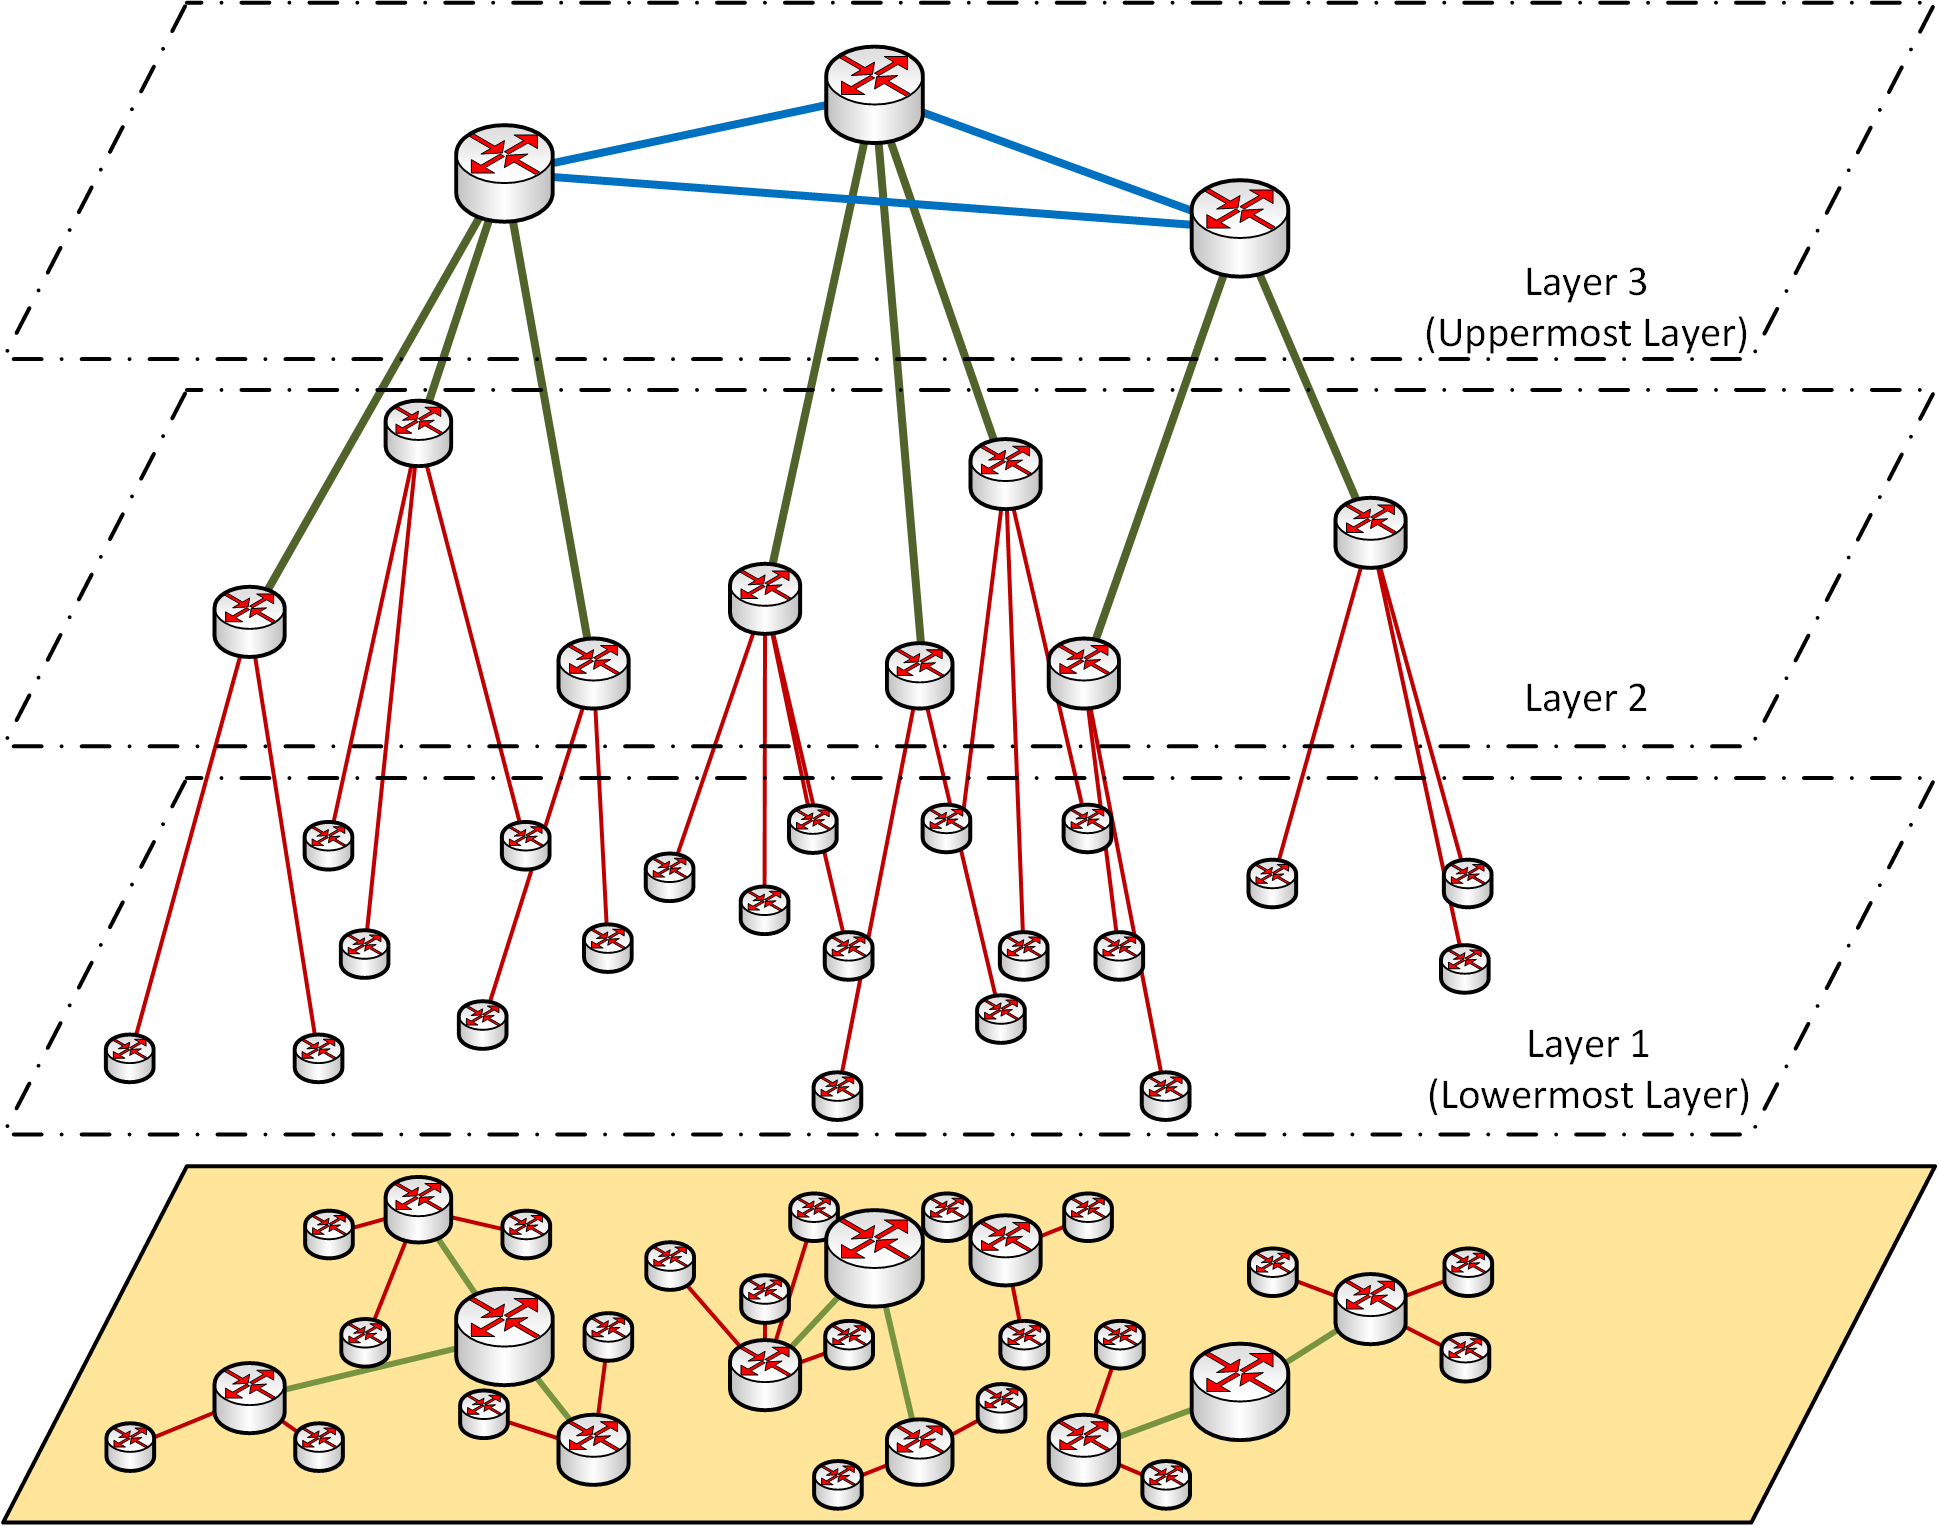
\includegraphics[width=15cm]{graphics/one_to_one/network}}
      \caption{دید کلی از توپولوژی شبکه}
      \label{fig:network}
    \end{figure}

    برای مقدار $\eta$ هم ۰٫۹ را در نظر می‌گیریم و فرض می‌کنیم ضرفیت پردازشی منابع پردازشی لبه شبکه به صورت تصادفی در محدوده‌ی $[1200, 1400]$ توزیع شده‌اند.
    برای ضرفیت پردازشی منابع پردازشی ابری هم مقدار ثابت $1000$ را در نظر می‌گیریم.
    علاوه بر این $\alpha_s$ به صورت تصادفی در بازه $[1, 10]$ توزیع شده است.
    در این فصل، برای هر سرویس تاخیر در حدود چند میلی ثانیه خواهد بود.
    در نتیجه برای رسیدن به نتایج معنی دار فرض می‌کنیم که $\beta_s = (1-\omega_s)/\omega_s$ به صورت یکنواخت در بازه $[30,70]$ توزیع شده اند.
    
    فرض می‌کنیم که تعداد سرویس‌ها $N=300$ باشد و تعداد منابع پردازشی لبه شبکه ($M$) از ۳۹۰ تا ۱۰۰۰ تغییر کند.
    در این قسمت هزینه سرویس $s$ را $-U_s$ تعریف می‌کنیم. 
    در نتیجه میانگین هزینه سرویس‌ها برابر خواهد بود با $-U/N$.
    دو سناریو را در نظر می‌گیریم.
    در سناریو‌ی اول فرض می‌کنیم که فقط منابع پردازشی لبه شبکه وجود دارند ولی در سناریو دوم یک فراهم کننده ابری با ۴۰ منبع پردازشی هم در شبکه حضور دارد.
    
    \begin{figure}
      \centerline{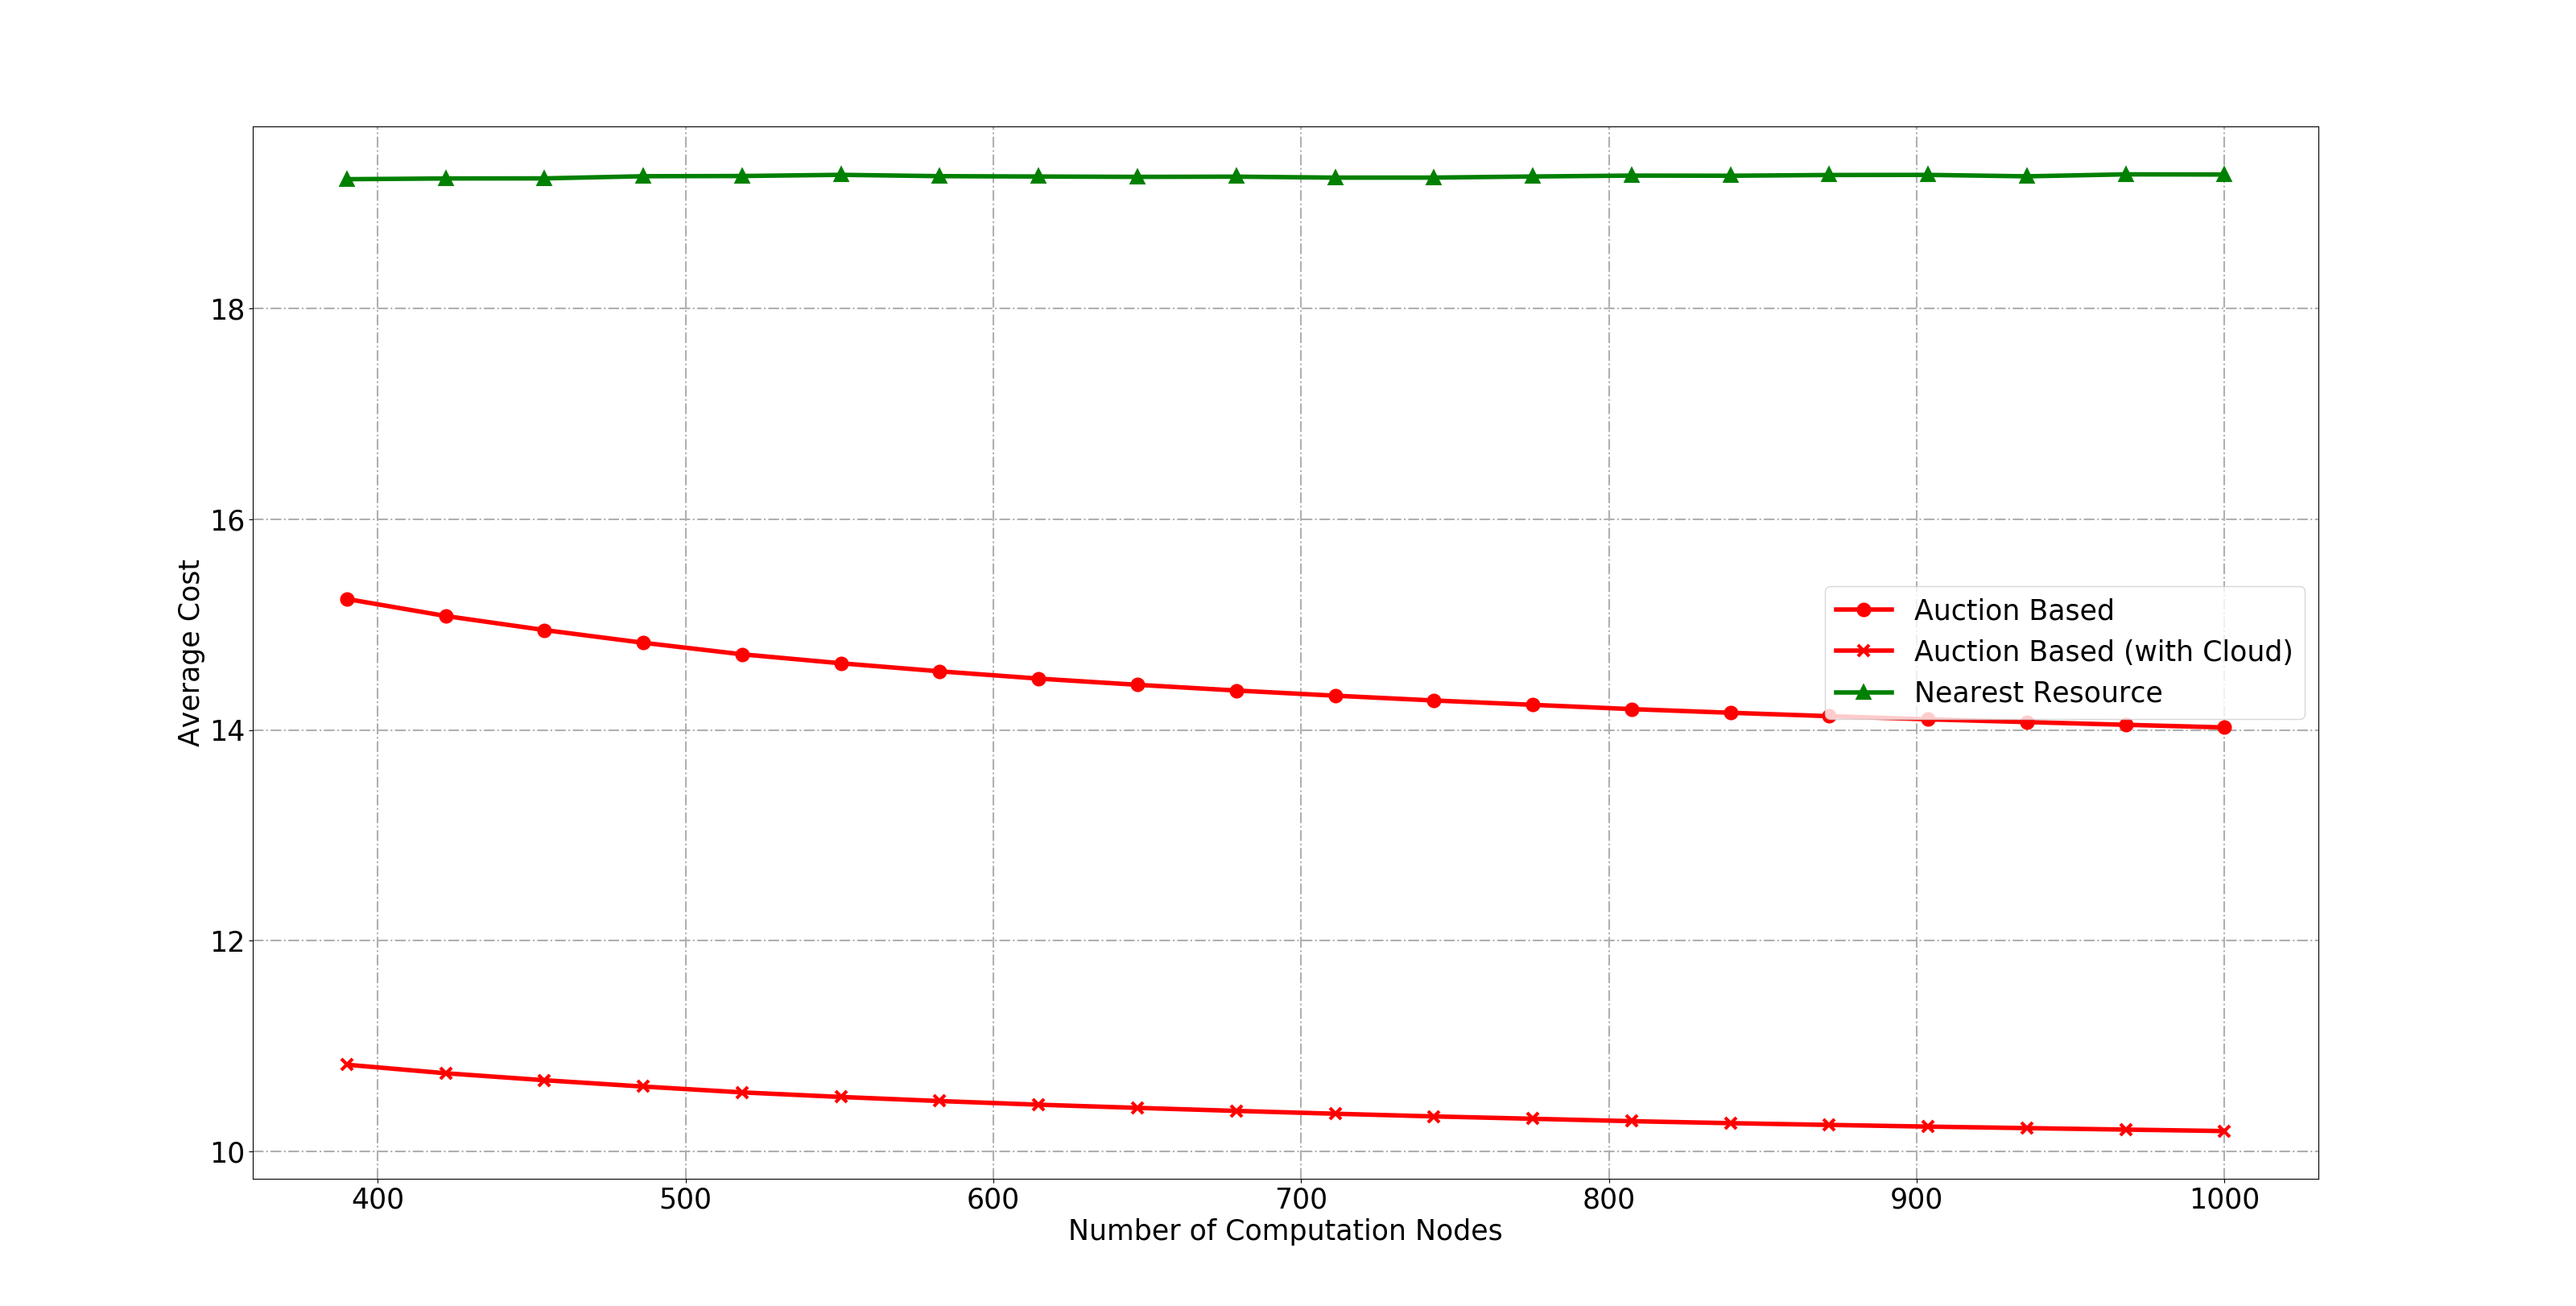
\includegraphics[width=17cm]{graphics/one_to_one/sim_1}}
      \caption{میانگین هزینه سرویس‌ها در برابر تعداد منابع پردازشی در لبه شبکه}
      \label{fig:ono_to_one:sim1}
    \end{figure}

    \cref{fig:ono_to_one:sim1} نتیجه شبیه سازی را برای سناریو‌های بیان شده نشان می‌دهد.
    برای مقایسه نتیجه، حاصل از اختصاص نزدیک‌ترین منبع پردازشی هم در شکل آورده شده است.
    در اختصاص نزدیک‌ترین منبع پردازشی، هر سرویس از نزدیک‌ترین منبع پردازشی به خود استفاده می‌کند.
    همان‌طور که از شکل مشخص است، تخصیص منابع مبتنی بر مزایده نتیجه بهتری نسبت به اختصاص نزدیک‌ترین منبع دارد.
    همان‌گونه که قبلا اشاره شد، زمانی که الگوریتم تخصیصی منابع پردازشی مبتنی بر حراج پایان می‌یابد، $U$ حداکثر به اندازه‌ی $N\epsilon$ با مقدار بیشینه فاصله دارد.
    بنابراین در هنگامی که الگوریتم پایان می‌یابد میانگین هزینه سرویس‌ها حداکثر به اندازه $\epsilon$ با مقدار کمینه فاصله دارد.
    در نتیجه برای مقادیر کوچک $\epsilon$ میانگین هزینه‌ها مقداری نزدیک به بهینه را خواهد داشت.

    از \cref{fig:ono_to_one:sim1} می‌توان استنباط کرد که با افزایش تعداد منابع پردازشی، میانگین هزینه‌ی سرویس‌ها کاهش پیدا می‌کند.
    افزایش تعداد منابع پردازشی باعث افزایش احتمال یافتن منبع پردازشی بهتر برای هر سرویس می‌شود پس کاهش هزینه نتیجه‌ای قابل قبول برای افزایش تعداد منابع پردازشی می‌باشد.
    نکته‌ی دیگری که می‌توان از این شکل برداشت کرد این است که با افزایش تعداد گره‌های پردازشی فاصله‌ی بین میانگین هزینه سرویس‌ها در سناریو‌ی با فراهم کننده منبع پردازشی ابری با بدون حضور آن به هم نزدیک می‌شود.
    دلیلی که می‌توان برای آن تصور کرد این است که با افزایش تعداد گره‌های پردازشی لبه شبکه احتمال اینکه سرویس‌ها، گره‌های پردازشی لبه شبکه را انتخاب کنند بیشتر می‌شود در نتیجه سرویس‌های کمتری از منابع پردازشی ابری استفاده خواهند کرد.
    با کاهش تعداد سرویس‌هایی که از منابع پردازشی ابری استفاده می کنند، اثر آن‌ها در میانگین هزینه سرویس‌ها کاهش پیدا می‌کند.
    در نتیجه تفاوت دو سناریو کاهش پیدا می‌کند.

    \begin{figure}
      \centerline{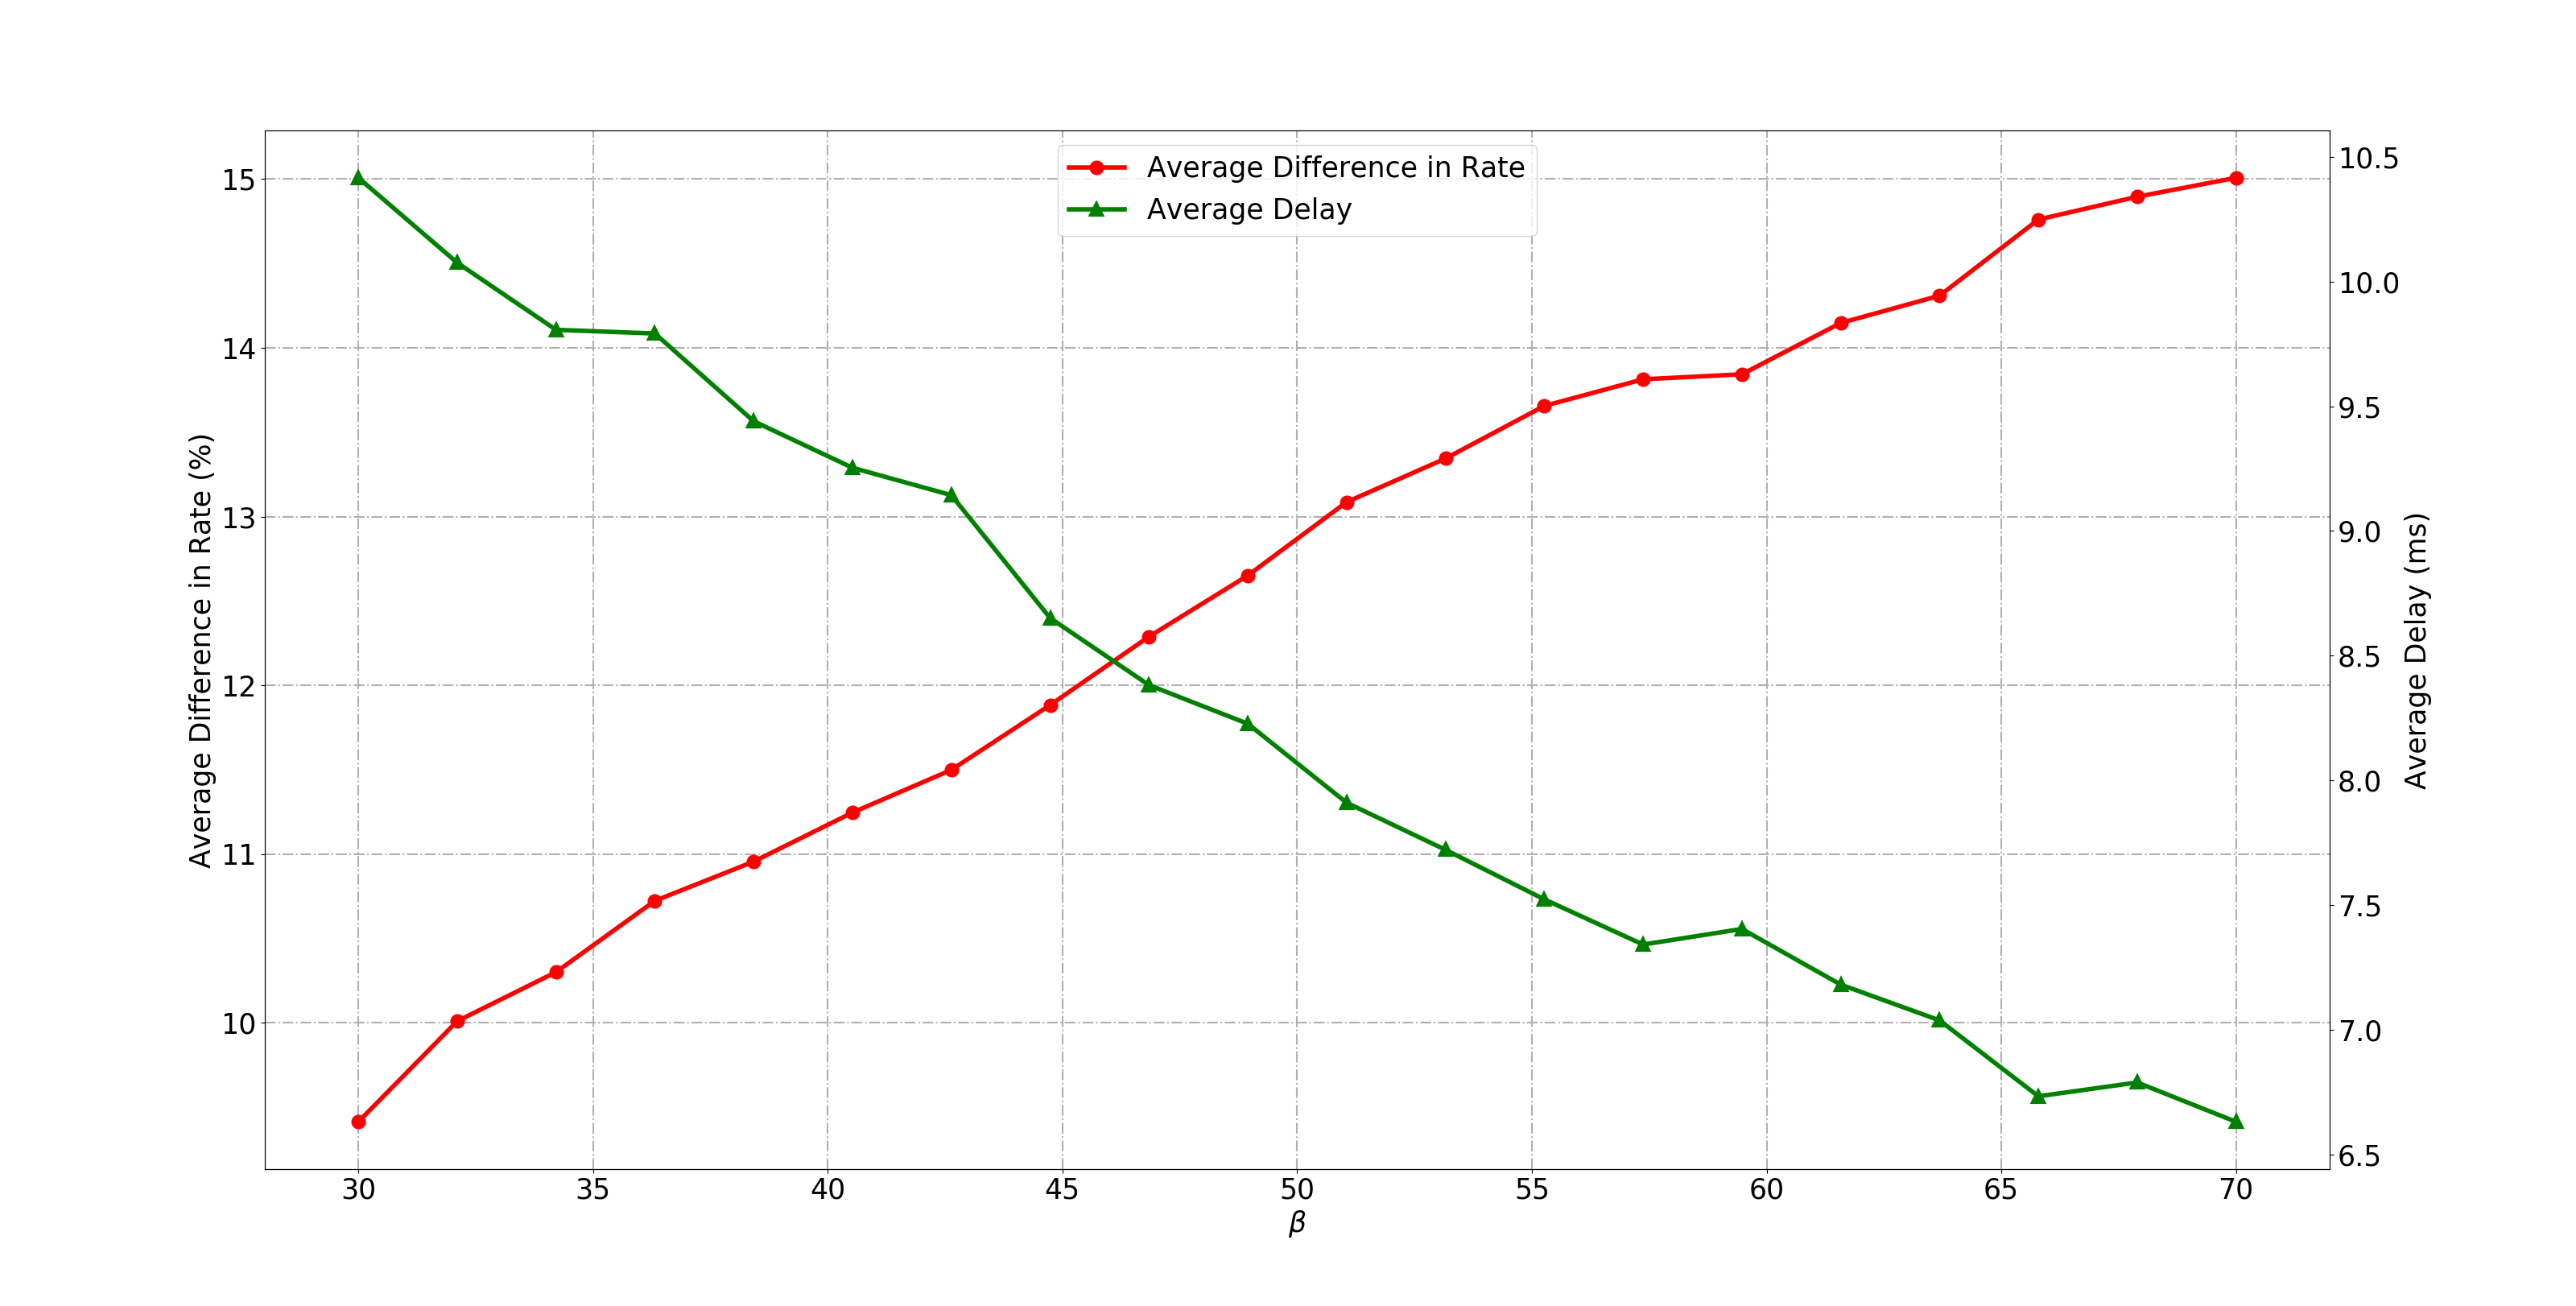
\includegraphics[width=17cm]{graphics/one_to_one/sim_2}}
      \caption{تاثیر $\beta$ بر تاخیر و اختلاف نرخ بهینه با نرخ مطلوب برای یک سرویس}
      \label{fig:ono_to_one:sim2}
    \end{figure}

    \cref{fig:ono_to_one:sim2} اثر $\beta$ روی میانگین تاخیر و میانگین اختلاف بین نرخ مطلوب و نرخ بهینه را برای یک سرویس نشان می‌دهد.
    در این شکل پارامتر‌های یاد شده برای $\beta \in [30, 70]$ رسم شده‌اند.
    در این‌جا فرض شده که همه پارامتر‌ها مانند قسمت قبل هستند و فرض شده که تأمین کننده‌ی منابع پردازشی ابری در شبکه حضور دارد.
    همان طور که قبلا بیان شد، $\beta$ بیان کننده نسبت اهمیت تاخیر به اختلاف نرخ مطلوب با نرخ بهینه است.
    به همین دلیل با افزایش $\beta$، اختلاف نرخ افرایش و تاخیر کاهش پیدا می‌کند.
    
    \begin{figure}
      \centerline{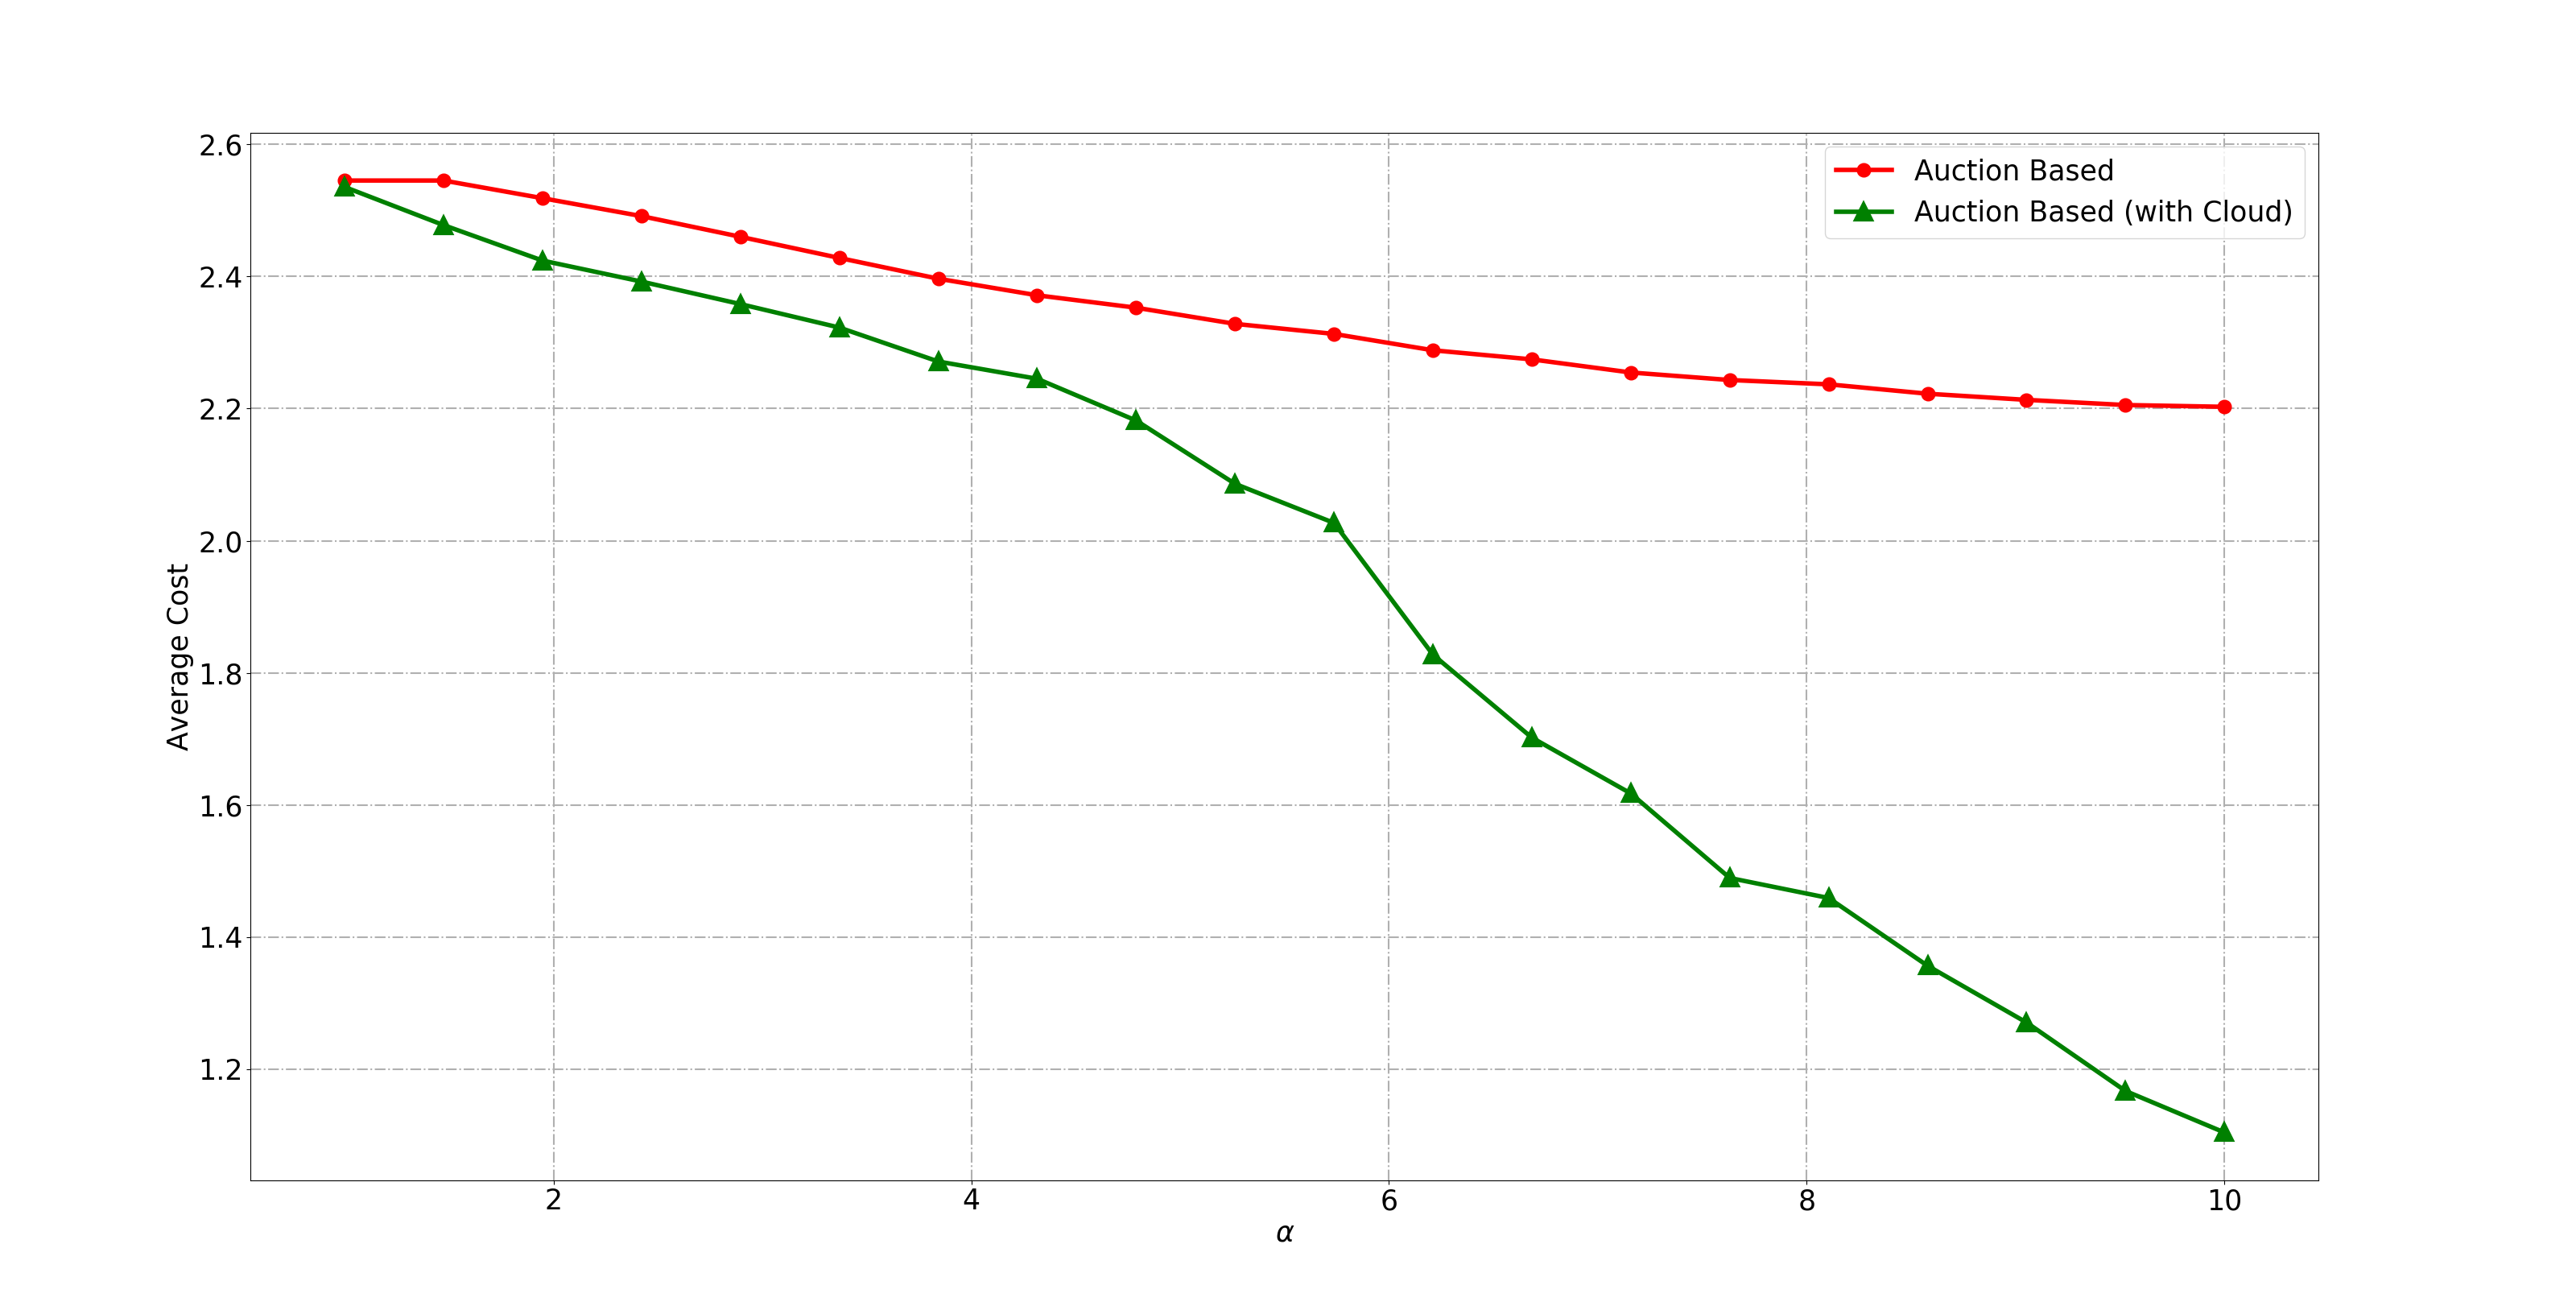
\includegraphics[width=17cm]{graphics/one_to_one/sim_3}}
      \caption{تاثیر $\alpha$ بر میانگین هزینه سرویس‌ها}
      \label{fig:ono_to_one:sim3}
    \end{figure}

    در \cref{fig:ono_to_one:sim3} تاثیر تغییر $\alpha_s$ بر روی هزینه یک سرویس‌ بررسی شده‌است.
    برای مقایسه، به جای رسم $U_s$ برای سرویس، $-U_s/\alpha_s$ رسم شده‌است.
    واضح است که افزایش $\alpha_s$، باعث افزایش اثر تاخیر و اختلاف نرخ مطلوب و نرخ بهینه سرویس $s$ در تابع هدف بهینه سازی می‌شود.
    در نتیجه انتظار داریم با افزایش $\alpha_s$، $U_s/\alpha_s$ افزایش پیدا کند که \cref{fig:ono_to_one:sim3} این موضوع را تایید می‌کند.

    \begin{figure}
      \centerline{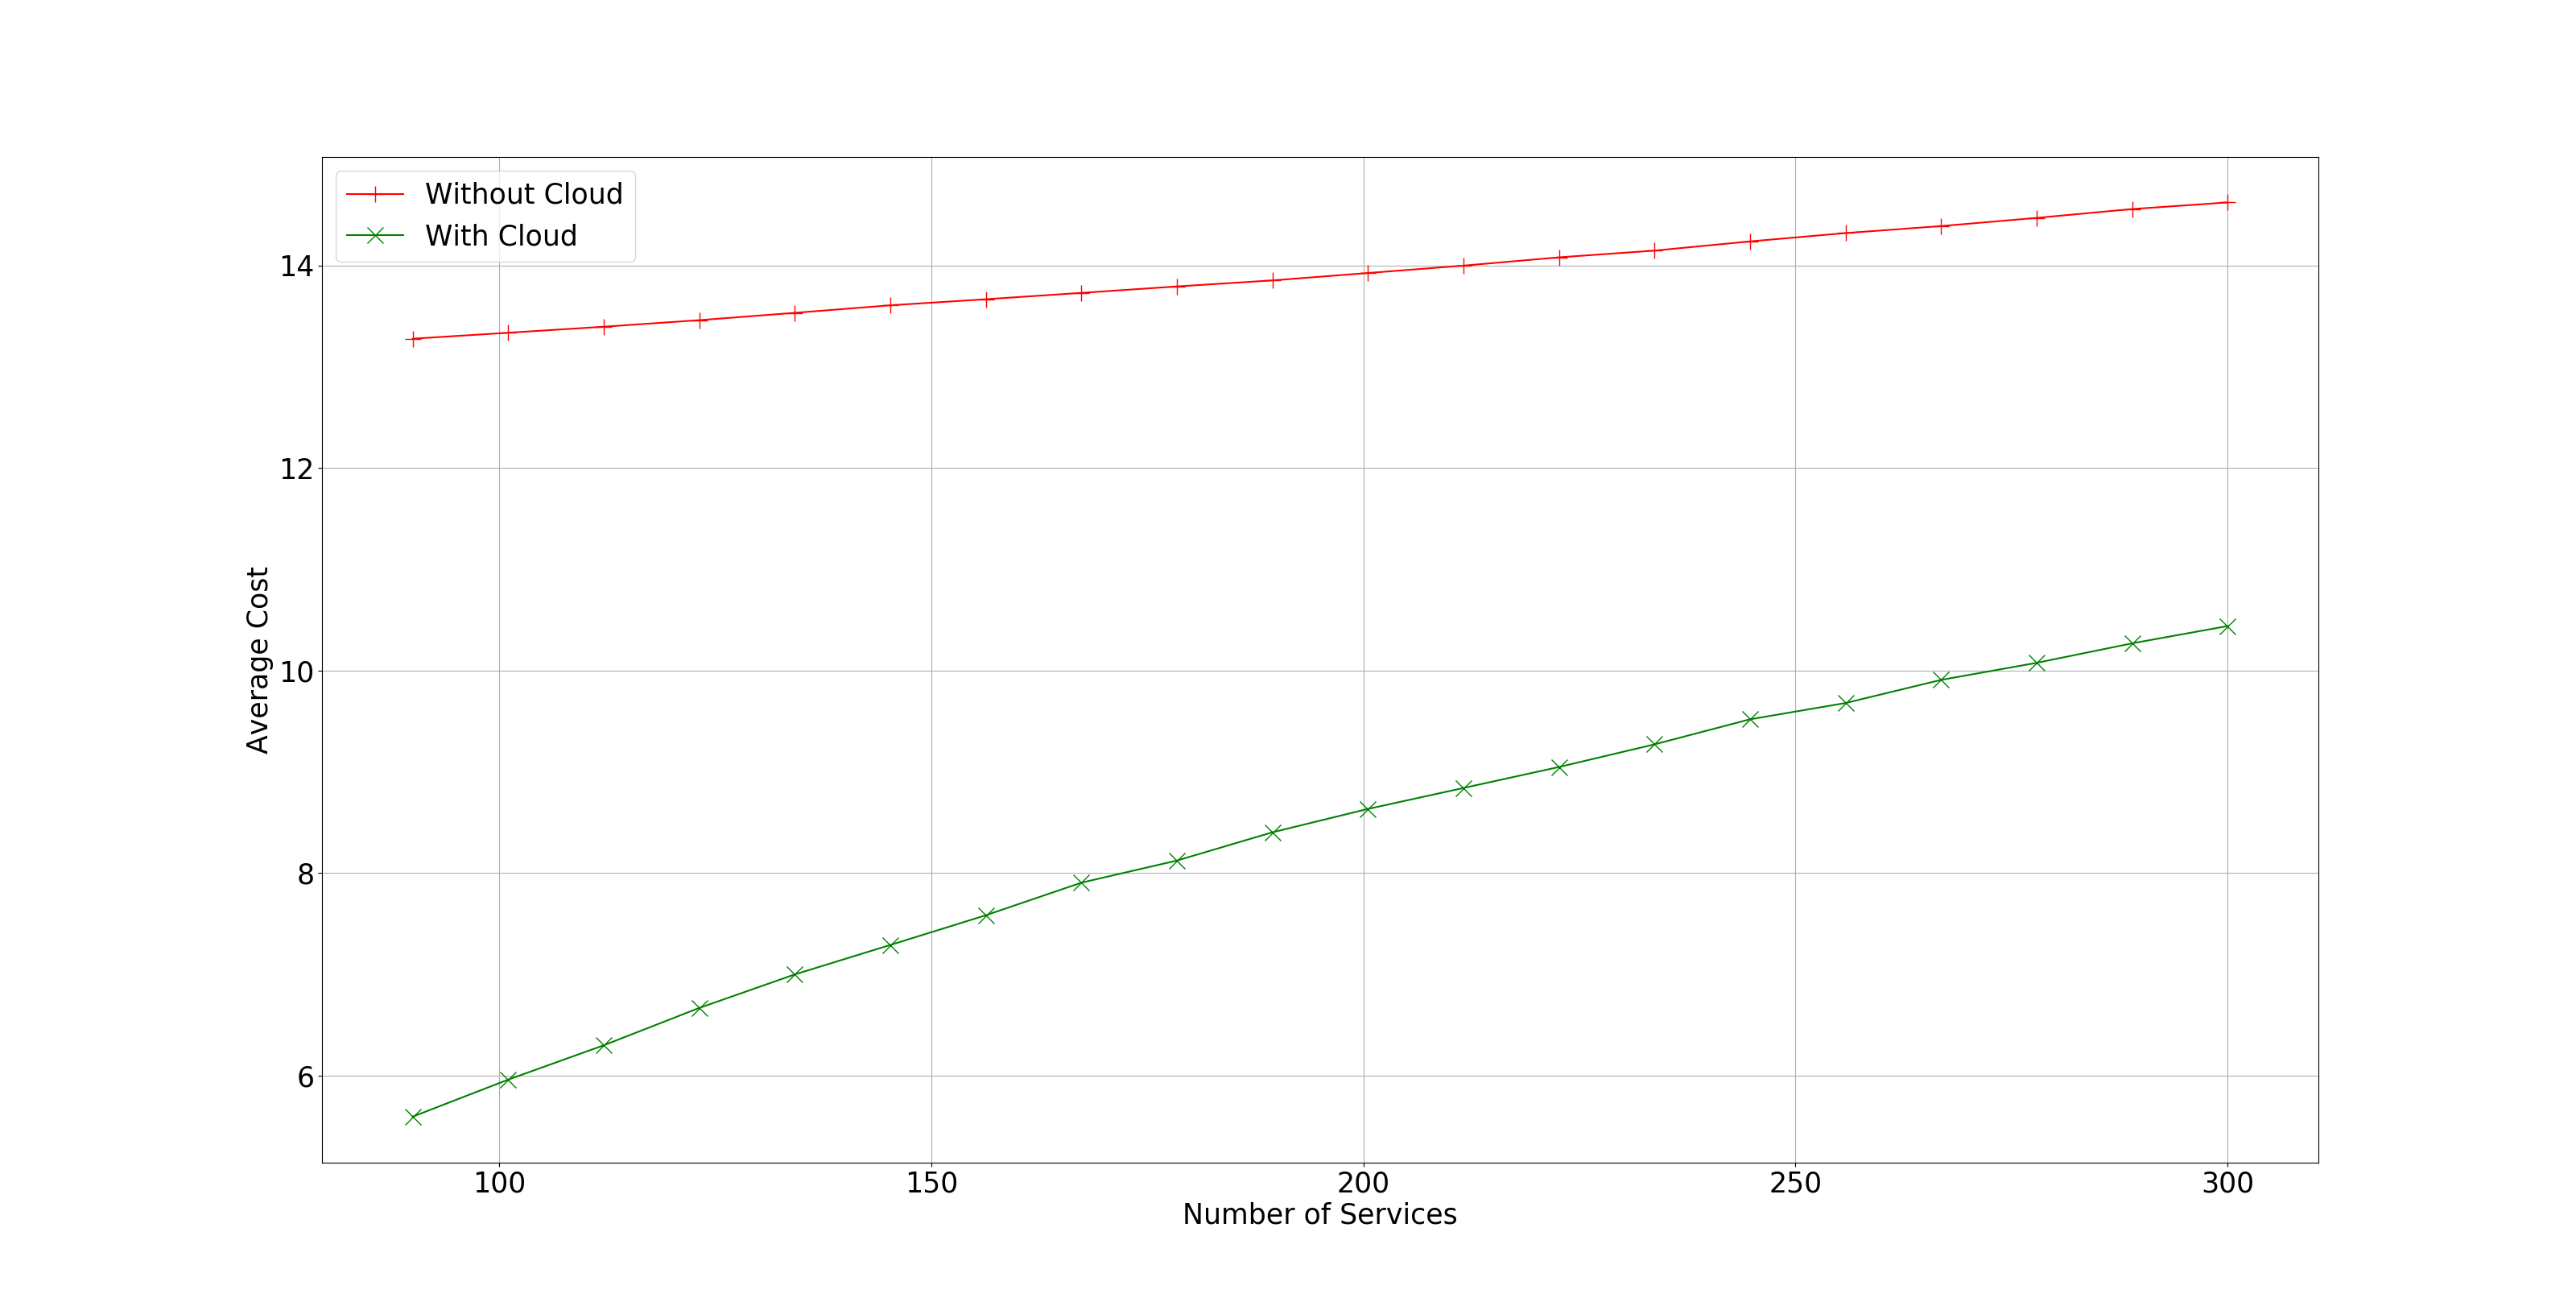
\includegraphics[width=17cm]{graphics/one_to_one/sim_4}}
      \caption{تاثیر تعداد سرویس‌ها بر میانگین هزینه سرویس‌ها}
      \label{fig:ono_to_one:sim4}
    \end{figure}

    \cref{fig:ono_to_one:sim4} تاثیر تعداد سرویس‌ها بروی روی میانگین هزینه سرویس‌ها را وقتی تعداد منابع پردازشی ثابت است،‌نشان می‌دهد.
    واضح است که با ثابت بودن منابع پردازشی، افزایش تعداد سرویس‌ها باعث افزایش رقابت برای یافتن بهترین منبع پردازشی می‌شود.
    در نتیجه احتمال دریافت بهترین منبع توسط منابع پردازشی کم‌تر می‌شود.

    \begin{figure}[H]
      \centerline{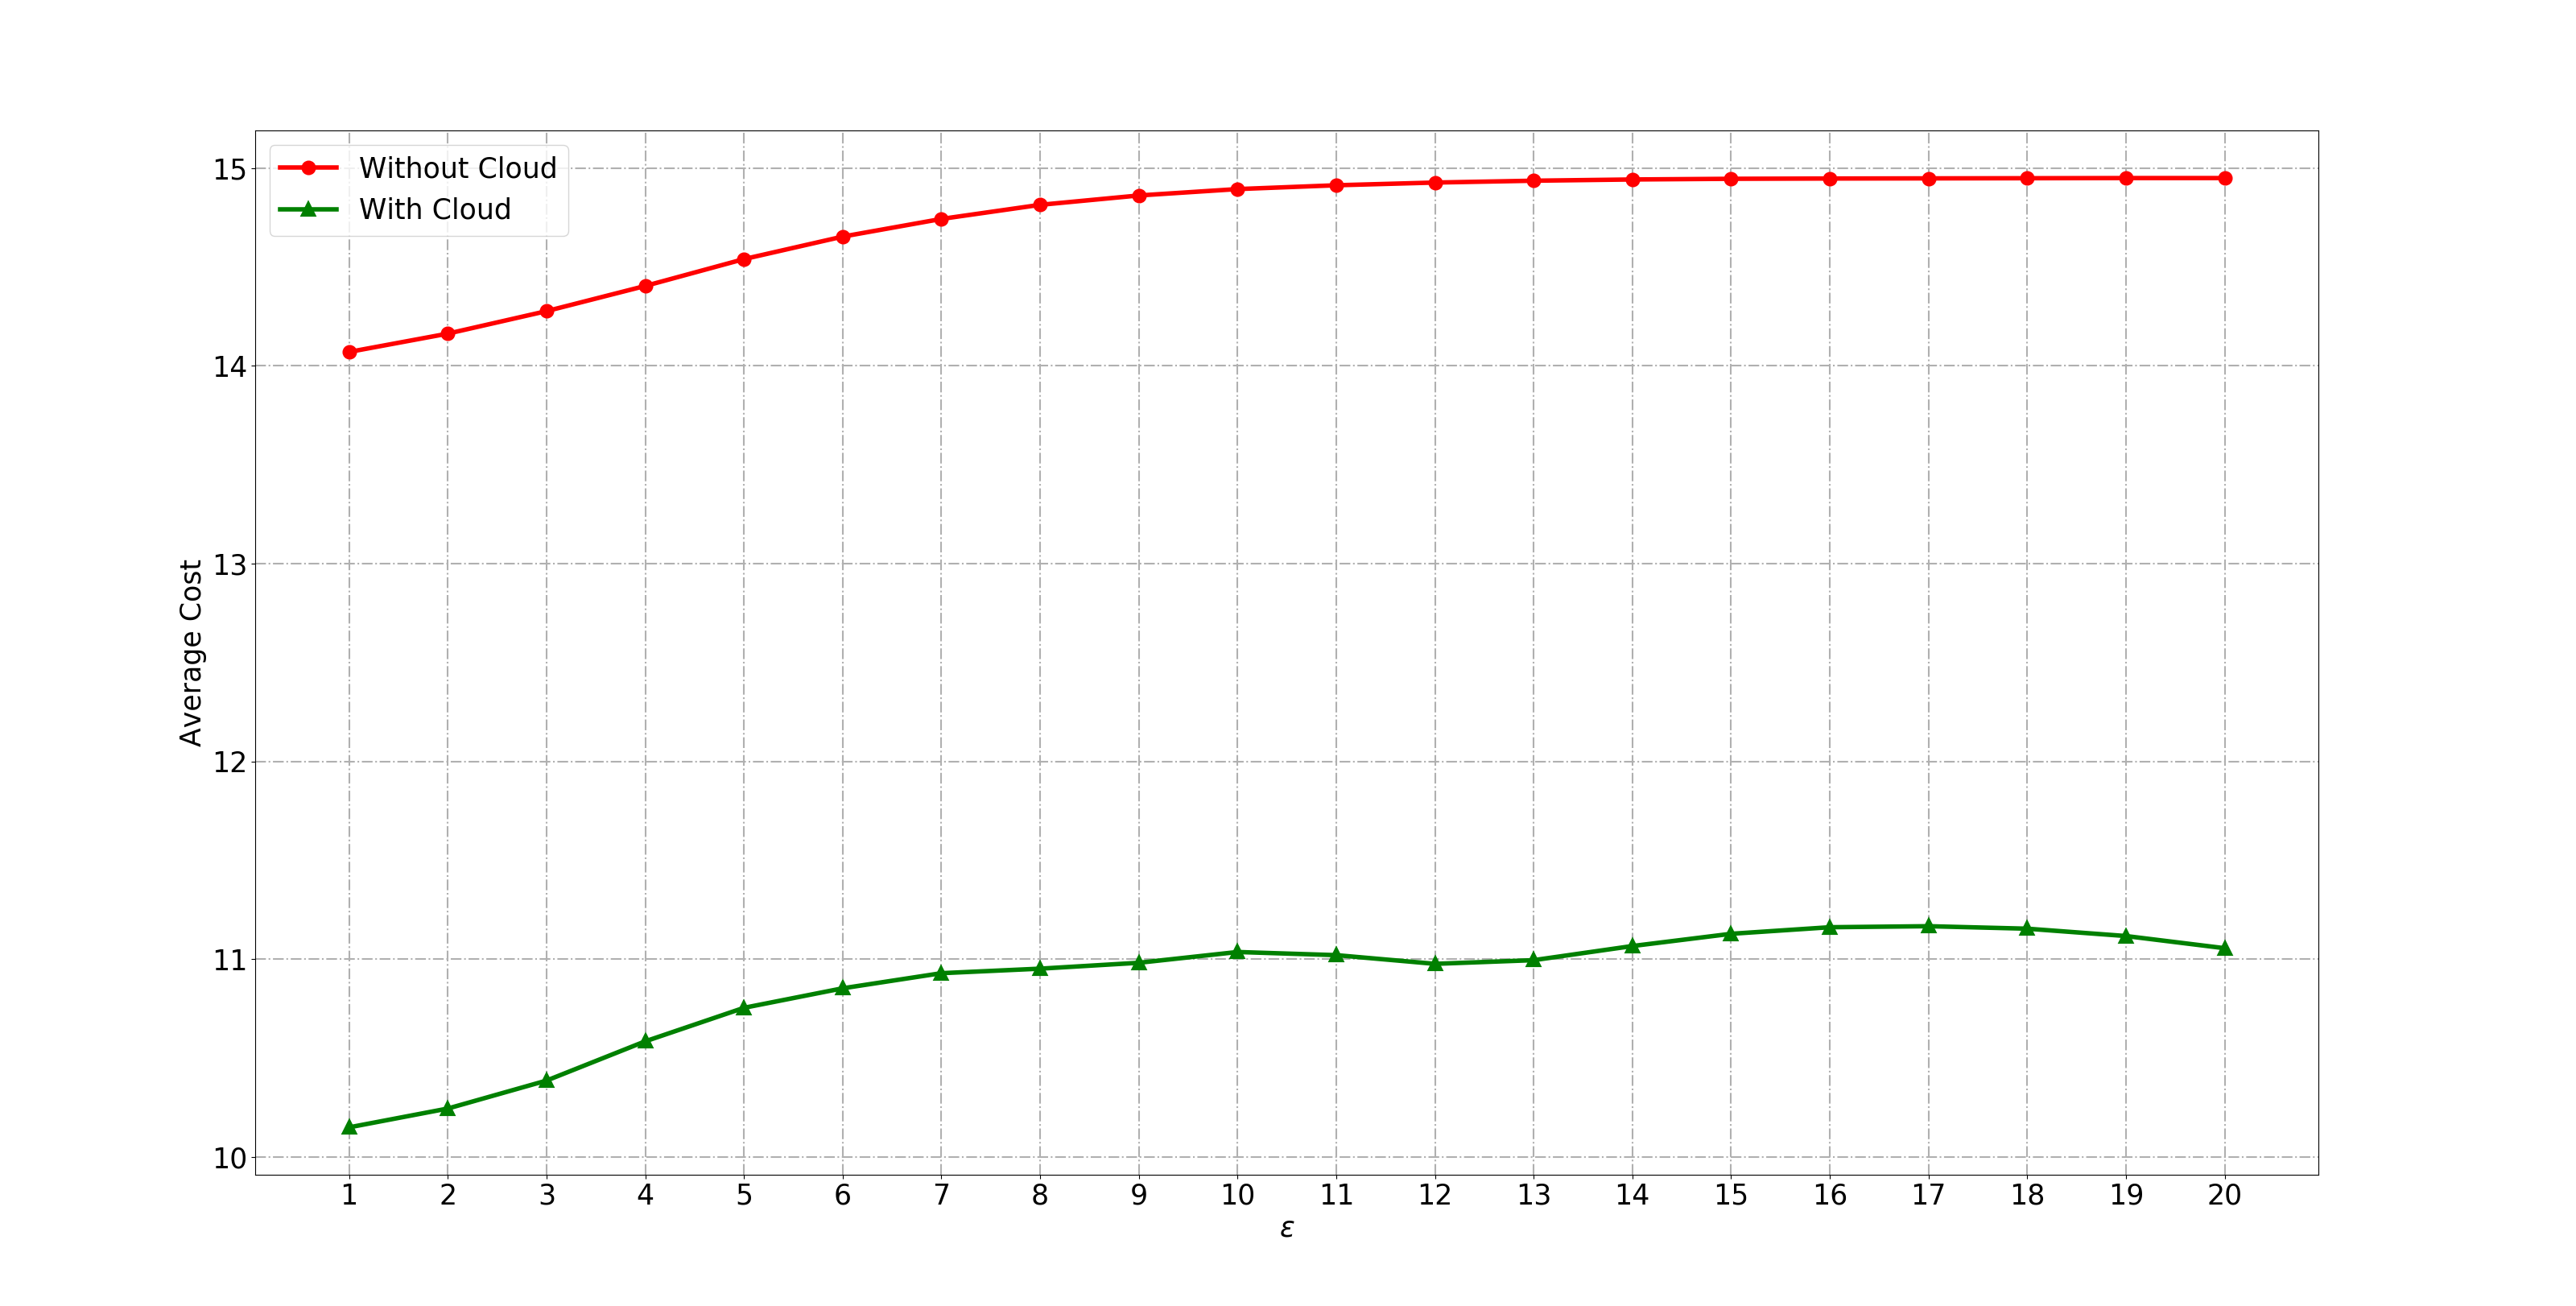
\includegraphics[width=17cm]{graphics/one_to_one/sim_5}}
      \caption{تاثیر $\epsilon$ بر میانگین ارزش همه‌ی سرویس‌ها}
      \label{fig:ono_to_one:sim5}
    \end{figure}

    در انتها در \cref{fig:ono_to_one:sim5} تاثیر $\epsilon$ بر نتیجه تخصیص منابع مشاهده می‌شود.
    مطابق مطالب بیان شده درباره‌ی روش تخصیص منابع مبتنی بر حراج با افزایش $\epsilon$ حد اکثر فاصله‌ی تخصیص منابع با مقدار بهینه بیشتر می‌شود و \cref{fig:ono_to_one:sim5} این موضوع را تأیید می‌کند.

  \section{جمع‌بندی و نتیجه‌گیری}
    در این فصل صورت مسئله تخصیص منابع پردازشی به صورت یک به یک برای سرویس‌های اینترنت اشیاء در یک شبکه بررسی شد.
    سپس الگوریتمی مبتنی بر مزایده معرفی  شد که مسئله فوق را در زمان قابل قبول حل می‌کند.
    پس از آن همگرایی، پیچیدگی و بهینگی الگوریتم مبتنی بر مزایده بررسی شد که نشان می‌داد که این الگوریتم، الگوریتم مناسبی برای استفاده در تخصیص منابع در شبکه اینترنت اشیاء است.
    در انتها نتیجه شبیه‌سازی‌ برای بررسی کارایی تخصیص منابع پردازشی توسط مزایده ارائه شد.
